\chapter{Analyzing QMCPACK data}
\label{chap:analyzing}

\section{Using the qmca tool to obtain total energies and related quantities}
\label{sec:qmca}

The \texttt{qmca} tool is the primary means of analyzing scalar valued 
data generated by QMCPACK.  Output files that contain scalar valued data 
are \texttt{*.scalar.dat} and \texttt{*.dmc.dat} (see chapter 
\ref{chap:output_overview} for a detailed description of these files).
Quantities that are available for analysis in \texttt{*.scalar.dat} files 
include the local energy and its variance, the kinetic energy, 
the potential energy and its components,
the acceptance ratio, and the average cpu time spent per block, among 
others.  The \texttt{*.dmc.dat} files provide information regarding 
the DMC walker population in addition to the local energy.  

Basic capabilities of \texttt{qmca} include calculating mean values 
and associated error bars, processing multiple files at once in batched 
fashion, performing twist averaging, plotting mean values by series, 
and plotting traces (per block or step) of the underlying data.  
These capabilities are explained with accompanying examples in the 
following subsections.

To use \texttt{qmca}, installations of Python and NumPy must be 
present on the local machine.  For graphical plotting, the matplotlib module 
must also be available.

An overview of all supported input flags to \texttt{qmca} can be 
obtained by typing ``\texttt{qmca}'' at the command line with no 
other inputs (also try ``\texttt{qmca -x}'' for a short list of examples):

\begin{shade}
>qmca
  no files provided, please see help info below 
  
  Usage: qmca [options] [file(s)]
  
  Options:
    --version             show program's version number and exit
    -v, --verbose         Print detailed information (default=False).
    -q QUANTITIES, --quantities=QUANTITIES
                          Quantity or list of quantities to analyze.  See names
                          and abbreviations below (default=all).
    -u UNITS, --units=UNITS
                          Desired energy units.  Can be Ha (Hartree), Ry
                          (Rydberg), eV (electron volts), kJ_mol (k.
                          joule/mole), K (Kelvin), J (Joules) (default=Ha).
    -e EQUILIBRATION, --equilibration=EQUILIBRATION
                          Equilibration length in blocks (default=auto).
    -a, --average         Average over files in each series (default=False).
    -w WEIGHTS, --weights=WEIGHTS
                          List of weights for averaging (default=None).
    -b, --reblock         (pending) Use reblocking to calculate statistics
                          (default=False).
    -p, --plot            Plot quantities vs. series (default=False).
    -t, --trace           Plot a trace of quantities (default=False).
    -h, --histogram       (pending) Plot a histogram of quantities
                          (default=False).
    -o, --overlay         Overlay plots (default=False).
    --legend=LEGEND       Placement of legend.  None for no legend, outside for
                          outside legend (default=upper right).
    --noautocorr          Do not calculate autocorrelation. Warning: error bars
                          are no longer valid! (default=False).
    --noac                Alias for --noautocorr (default=False).
    --sac                 Show autocorrelation of sample data (default=False).
    --sv                  Show variance of sample data (default=False).
    -i, --image           (pending) Save image files (default=False).
    -r, --report          (pending) Write a report (default=False).
    -s, --show_options    Print user provided options (default=False).
    -x, --examples        Print examples and exit (default=False).
    --help                Print help information and exit (default=False).
    -d DESIRED_ERROR, --desired_error=DESIRED_ERROR
                          Show number of samples needed for desired error bar
                          (default=none).
    -n PARTICLE_NUMBER, --enlarge_system=PARTICLE_NUMBER
                          Show number of samples needed to maintain error bar on
                          larger system: desired particle number first, current
                          particle number second (default=none) 
\end{shade}

\subsection{Obtaining a statistically correct mean and error bar}
\label{sec:qmca_mean_error}
A rough guess at the mean and error bar of the local energy can be 
obtained in the following way with \texttt{qmca}:
\begin{shade}
>qmca -q e qmc.s000.scalar.dat 
qmc  series 0  LocalEnergy           =  -45.876150 +/- 0.017688 
\end{shade}
\noindent
In this case the VMC energy of an 8 atom cell of diamond is estimated 
to be $-45.876(2)$ Hartrees.  This rough guess should not be used 
for production-level or publication quality estimates.

To obtain production-level results, the underlying data should first  
inspected visually to ensure that all data included in the averaging 
can be attributed to a distribution sharing the same mean.  The first 
steps of essentially any Monte Carlo calculation (the ``equilibration 
phase'') do not belong to the equilibrium distribution and should be 
excluded from estimates of the mean and its error bar.

We can plot a data trace (``\texttt{-t}'') of the local energy in the 
following way:
\begin{shade}
>qmca -t -q e -e 0 qmc.s000.scalar.dat
\end{shade}
\noindent
The ``\texttt{-e 0}'' part indicates that we do not want any data 
to be excluded from the calculation of averages initially.  The resulting 
plot is shown in Fig. \ref{fig:qmca_mean_error_trace}.  The unphysical 
equilibration period is visible on the left side of the plot.

Most of the data fluctuates around a well defined mean (consistent 
variations around a flat line).  This property is important to verify  
by plotting the trace for each QMC run. 

\begin{figure}
\begin{center}
\ifdefined\HCode
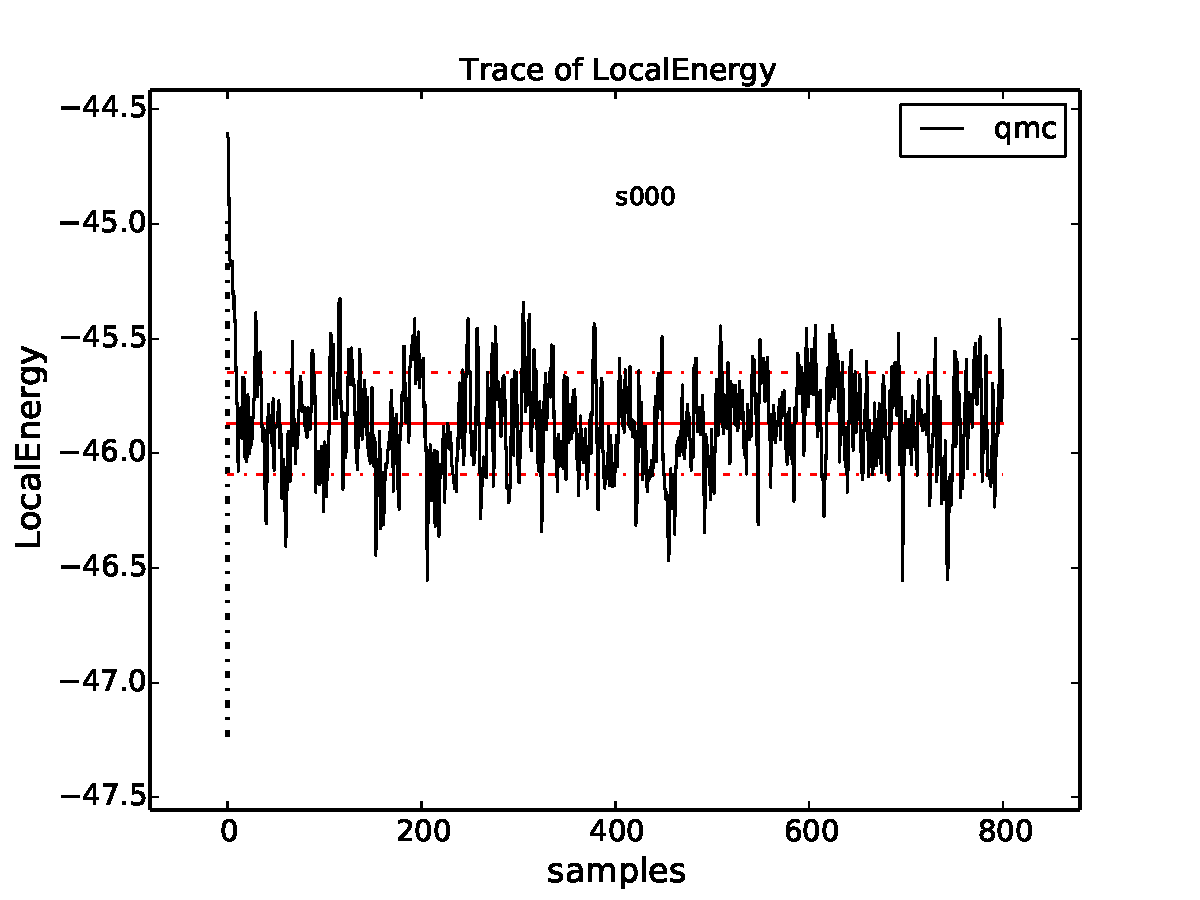
\includegraphics[trim = 0mm 0mm 0mm 0mm,clip,width=0.75\textwidth]{./figures/qmca_mean_error_trace.dmn}
\else
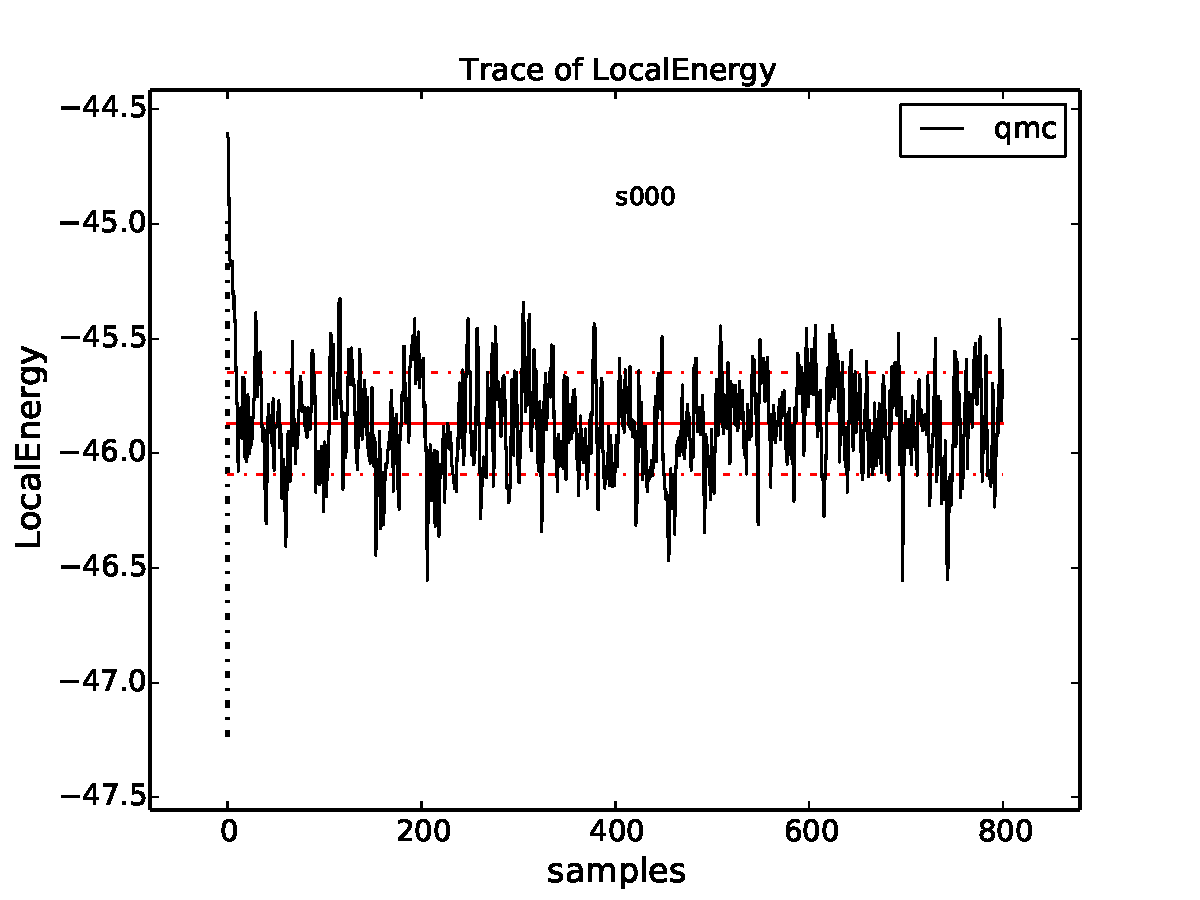
\includegraphics[trim = 0mm 0mm 0mm 0mm,clip,width=0.75\textwidth]{./figures/qmca_mean_error_trace.pdf}
\fi
\caption{Trace of the VMC local energy for an 8 atom cell of diamond generated with \texttt{qmca}.  The x-axis (``samples'') refers to the VMC block index in this case.}
\label{fig:qmca_mean_error_trace}
\end{center}
\end{figure}

If we exclude none of the equilibration data points, we get an 
erroneous estimate of $-45.870(2)$ Ha for the local energy:
\begin{shade}
>qmca -q e -e 0 qmc.s000.scalar.dat 
qmc  series 0  LocalEnergy           =  -45.870071 +/- 0.018072
\end{shade}
\noindent
The equilibration period is typically estimated by eye, though one should
check a few conservative values to ensure that the mean remains 
unaffected.  In this dataset, the equilibration appears to have been 
reached after 100 samples or so.  After excluding the first 100 
VMC blocks from the analysis we get:
\begin{shade}
>qmca -q e -e 100 qmc.s000.scalar.dat 
qmc  series 0  LocalEnergy           =  -45.877363 +/- 0.017432
\end{shade}
\noindent
This estimate ($-45.877(2)$ Ha) differs significantly from the 
$-45.870(2)$ Ha figure obtained from the full set of data, but it 
agrees with the rough estimate of $-45.876(2)$ Hartrees obtained 
with the abbreviated command (``\texttt{qmca -q e qmc.s000.scalar.dat}'').
This is because \texttt{qmca} makes a heuristic guess at the 
equilibration period and got it reasonably correct in this case. 
There are many cases where the heuristic guess fails and it should not 
be relied on for quality results.

We have so far obtained a statistically correct mean.  To obtain 
a statistically correct error bar it is best to include $\sim$100 or more 
statistically independent samples.  An estimate of the number 
of independent samples can be obtained by considering the 
autocorrelation time, which is essentially a measure of the number of 
samples that must be traversed before an uncorrelated/independent sample 
is reached.  We can get an estimate of the autocorrelation time 
in the following way:
\begin{shade}
>qmca -q e -e 100 qmc.s000.scalar.dat --sac
qmc  series 0  LocalEnergy           =  -45.877363 +/- 0.017432    4.8 
\end{shade}
\noindent
The flag ``\texttt{--sac}'' stands for (s)how (a)uto(c)orrelation.  
In this case the autocorrelation estimate is $4.8\approx 5$ samples. 
Since the total run contained 800 samples and we have excluded 100 of 
them, we can estimate the number of independent samples as 
$(800-100)/5=140$.  In this case, the error bar is expected to be 
estimated reasonably well.

Please keep in mind that the error bar represents the expected range
of the mean with a certainty of only $\sim 70\%$, i.e. it is a one
sigma error bar.  The actual mean value will lie outside the range
indicated by the error bar in one out of every three runs and in a set
of 20 runs one value can be expected to deviate from its estimate by
twice the error bar.


\subsection{Judging wavefunction optimization}
\label{sec:qmca_judge_opt}
Wavefunction optimization is a highly non-linear and sometimes 
sensitive process.  As such, there is a risk that systematic 
errors encountered at this stage of the QMC process can be propagated 
into subsequent (expensive) DMC runs unless they are guarded against 
with vigilance.

In this section we again consider an 8 atom cell of diamond, but 
now in the context of Jastrow optimization (one- and two-body terms). 
In optimization runs it is often preferable to use a large number 
of \texttt{warmupsteps} ($\sim 100$) so that equilibration bias does 
not propagate into the optimization process.  We can check that 
the added warmup has had its intended effect by again checking the 
local energy trace:
\begin{shade}
>qmca -t -q e *scalar*
\end{shade}
\noindent
The resulting plot can be found in Fig. \ref{fig:qmca_judge_opt}. 
In this case sufficient \texttt{warmupsteps} were used to exit 
the equilibration period before samples were collected and we can 
proceed without using the ``\texttt{-e}'' option with \texttt{qmca}.

\begin{figure}
\begin{center}
\ifdefined\HCode  
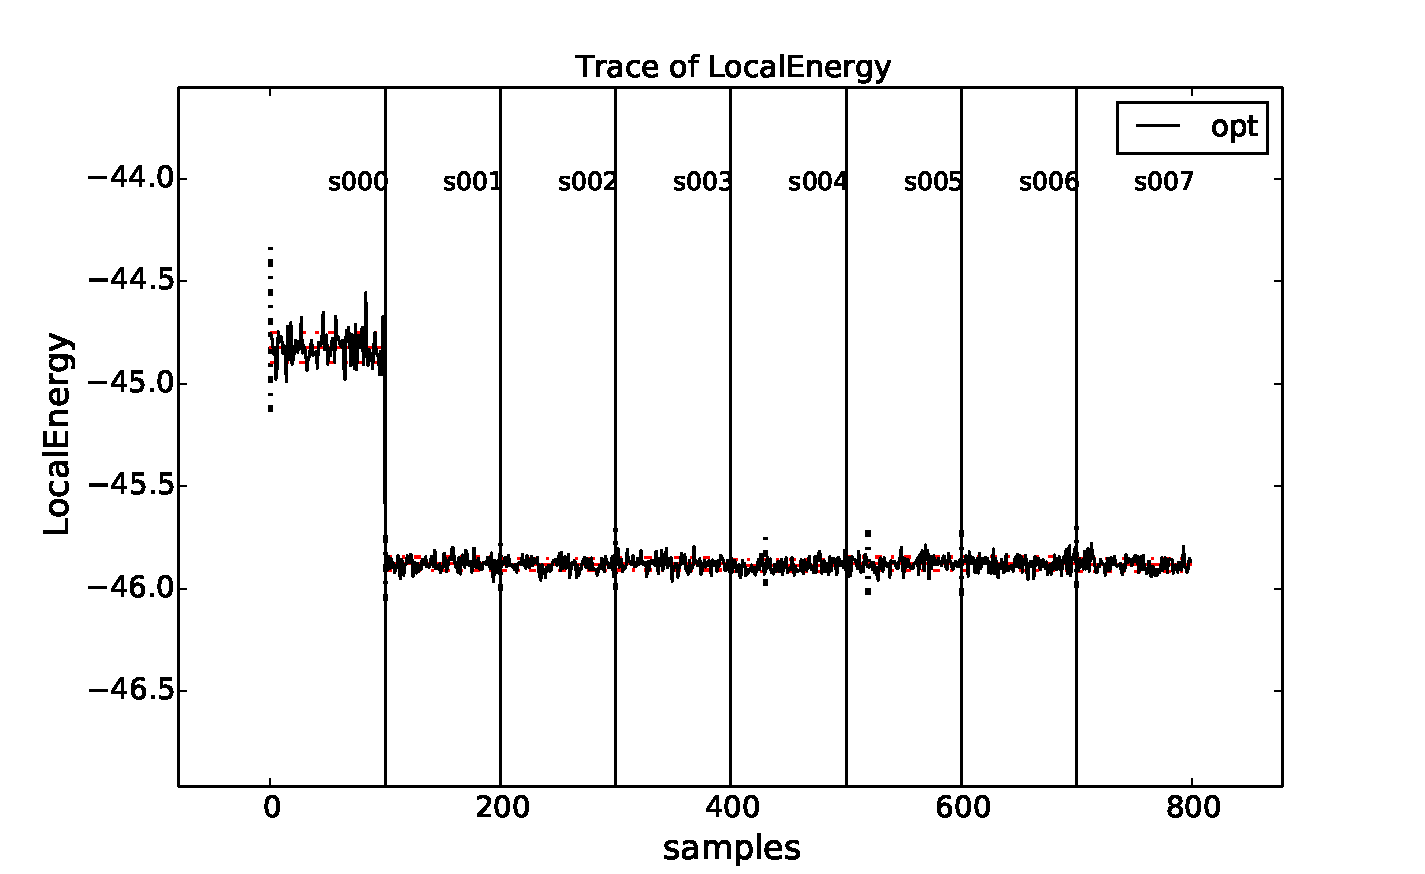
\includegraphics[trim = 0mm 0mm 0mm 0mm, clip,width=0.9\textwidth]{./figures/qmca_judge_opt.dmn}
\else
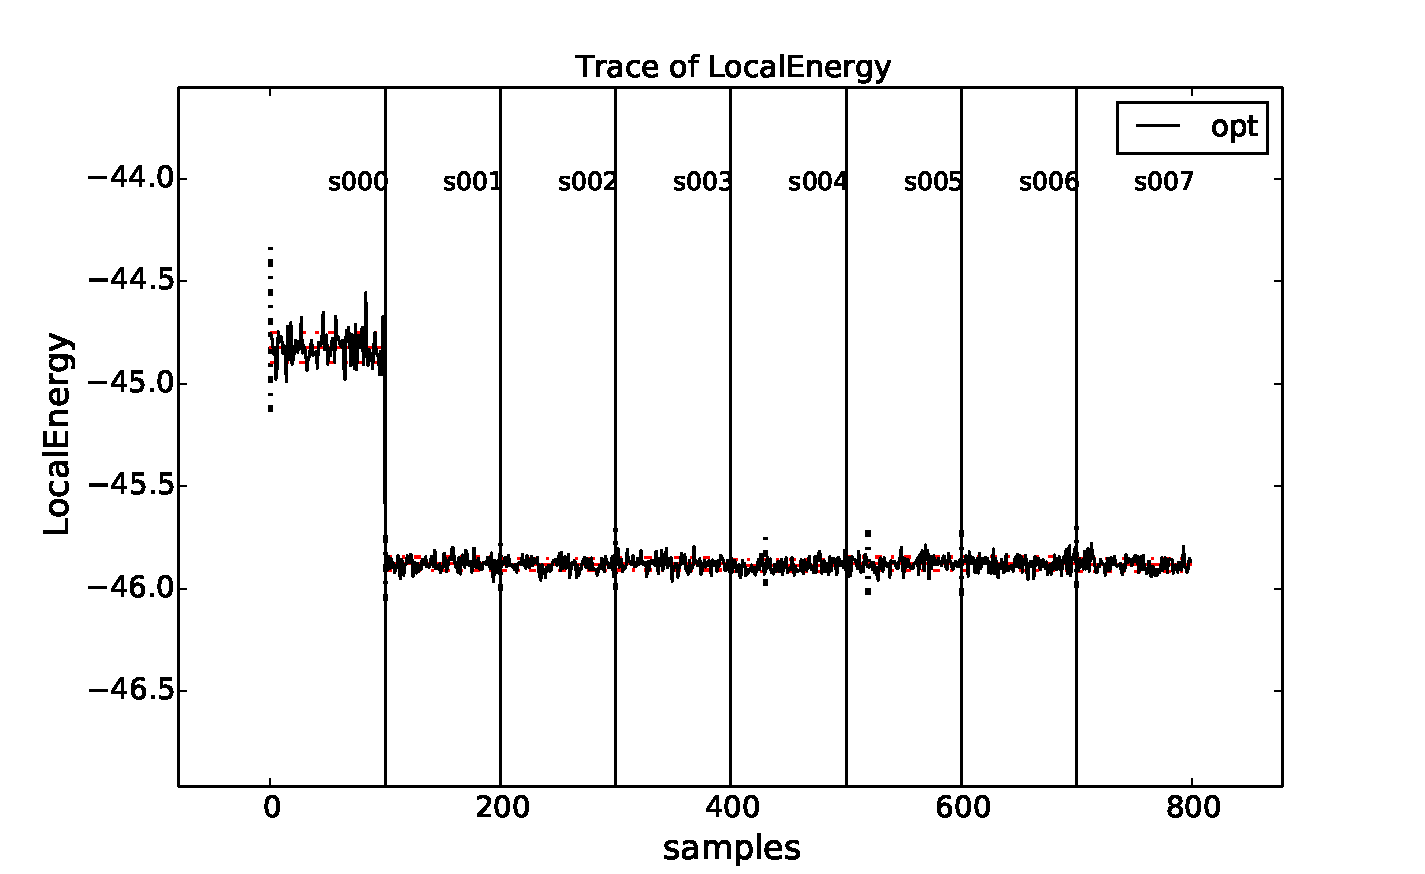
\includegraphics[trim = 0mm 0mm 0mm 0mm, clip,width=0.9\columnwidth]{./figures/qmca_judge_opt.pdf}
\fi
\end{center}
\caption{Trace of the local energy during one- and two-body Jastrow optimization for an 8 atom cell of diamond generated with \texttt{qmca}.  Data for each optimization cycle (QMCPACK series) is separated by a vertical black line.
}
\label{fig:qmca_judge_opt}
\end{figure}

After inspecting the trace, we should inspect the text output 
from \texttt{qmca}, now including the total energy and its variance:
\begin{shade}
>qmca -q ev opt*scalar.dat
                            LocalEnergy               Variance           ratio 
opt  series 0  -44.823616 +/- 0.007430   7.054219 +/- 0.041998   0.1574 
opt  series 1  -45.877643 +/- 0.003329   1.095362 +/- 0.041154   0.0239 
opt  series 2  -45.883191 +/- 0.004149   1.077942 +/- 0.021555   0.0235 
opt  series 3  -45.877524 +/- 0.003094   1.074047 +/- 0.010491   0.0234 
opt  series 4  -45.886062 +/- 0.003750   1.061707 +/- 0.014459   0.0231 
opt  series 5  -45.877668 +/- 0.003475   1.091585 +/- 0.021637   0.0238 
opt  series 6  -45.877109 +/- 0.003586   1.069205 +/- 0.009387   0.0233 
opt  series 7  -45.882563 +/- 0.004324   1.058771 +/- 0.008651   0.0231 
\end{shade}
\noindent
The flags ``\texttt{-q ev}'' requested the energy (\texttt{e}) and 
the variance (\texttt{v}).  For this combination of quantities, a 
third column (``\texttt{ratio}'') is printed containing the ratio 
of the variance and the absolute value of the local energy.
The variance/energy ratio is an intensive quantity and is useful  
to inspect regardless of the system under study.  Successful 
optimization of molecules and solids of any size generally result 
in comparable values for the variance/energy ratio. 

The first line of 
the output (``\texttt{series 0}'') corresponds to the local energy 
and variance of the system without a Jastrow factor (all Jastrow 
coefficients were initialized to zero in this case), reflecting the 
quality of the orbitals alone. For pseudopotential systems, a 
variance/energy ratio $>0.20$ Ha generally indicates there is a problem 
with the input orbitals that needs to be resolved prior to 
performing wavefunction optimization.  

The subsequent lines correspond to energies and variances of 
intermediate parameterizations of the trial wavefunction during 
the optimization process.  The output line containing 
``\texttt{opt  series 1}'', for example, corresponds to the trial 
wavefunction parameterized during the ``\texttt{series 0}'' step 
(the parameters of this wavefunction would be found in an output 
file matching \texttt{*s000*opt.xml}).  The first thing to check 
about the resulting optimization is again the variance/energy ratio. 
For pseudopotential systems, a variance/energy ratio $<0.03$ Ha is 
consistent with a trial wavefunction of production quality, and values 
of $0.01$ Ha are rarely obtainable for standard Slater-Jastrow 
wavefunctions.  By this metric, all parameterizations obtained for 
optimizations performed in series 0-6 are of comparable quality 
(note that the quality of the wavefunction obtained during optimization 
series 7 is effectively unknown).

A good way to further discriminate among the parameterizations is to 
plot the energy and variance as a function of series with \texttt{qmca}:
\begin{shade}
>qmca -p -q ev opt*scalar.dat
\end{shade}
\noindent
The ``\texttt{-p}'' option results in plots of means plus error bars 
vs. series for all requested quantities.
The resulting plots for the local energy and variance are shown 
in Fig. \ref{fig:qmca_opt_ev}.  In this case the resulting energies 
and variances are statistically indistinguishable for all optimization 
cycles.  

\begin{figure}
  \centering
  \ifdefined\HCode%
  \begin{tabularx}{1024pt}{X X}
    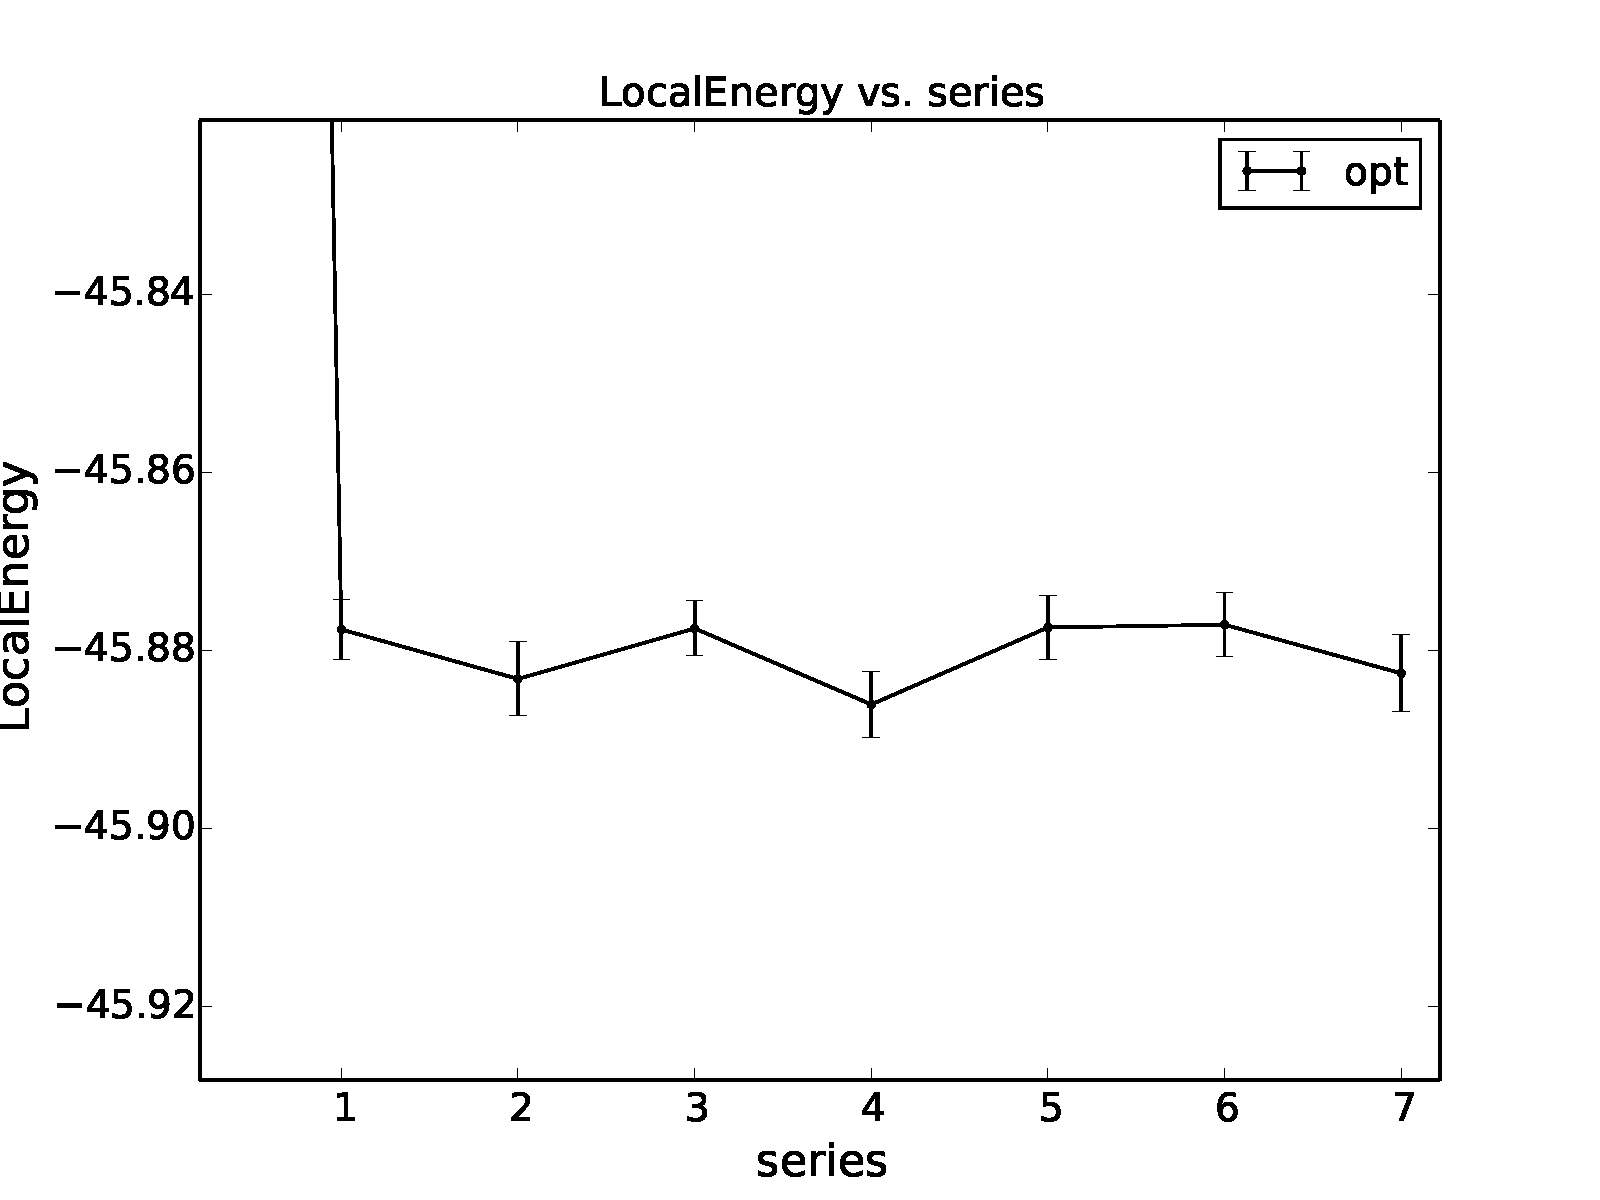
\includegraphics[trim=0mm 0mm 4mm 0mm,clip,width=512pt]{./figures/qmca_opt_energy.dmn}&
    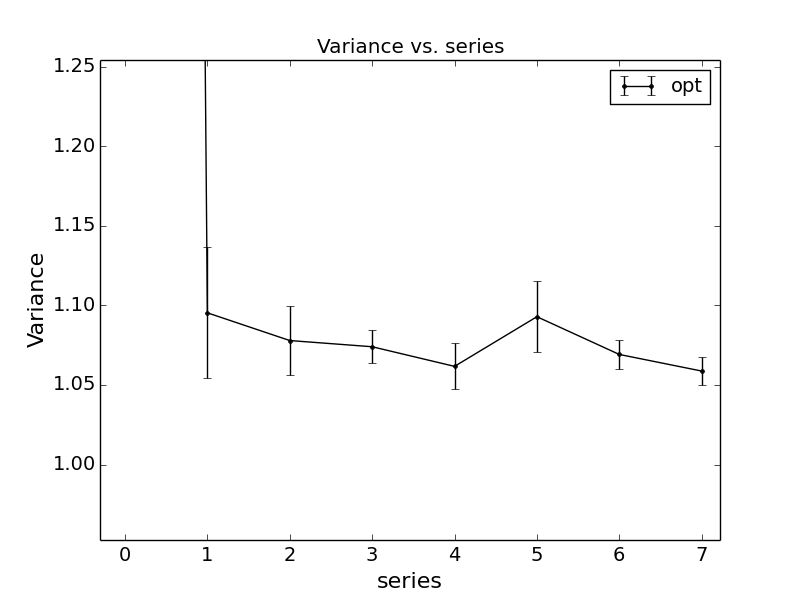
\includegraphics[trim=2mm 0mm 4mm 0mm,clip,width=512pt]{./figures/qmca_opt_variance.png}\\
  \end{tabularx}
\else%
  \begin{tabularx}{\textwidth}{X X}
    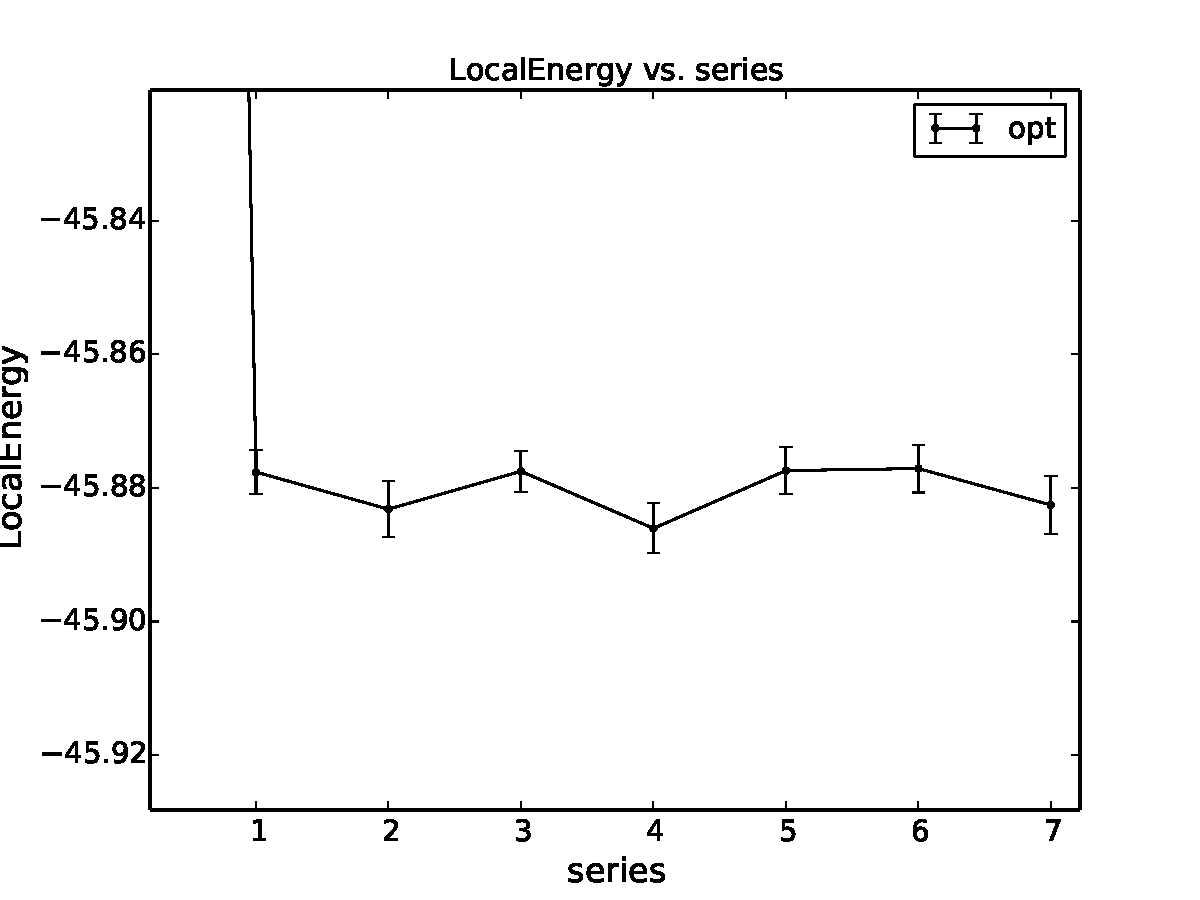
\includegraphics[trim=0mm 0mm 4mm 0mm,clip,width=0.47\textwidth]{./figures/qmca_opt_energy.pdf}&
    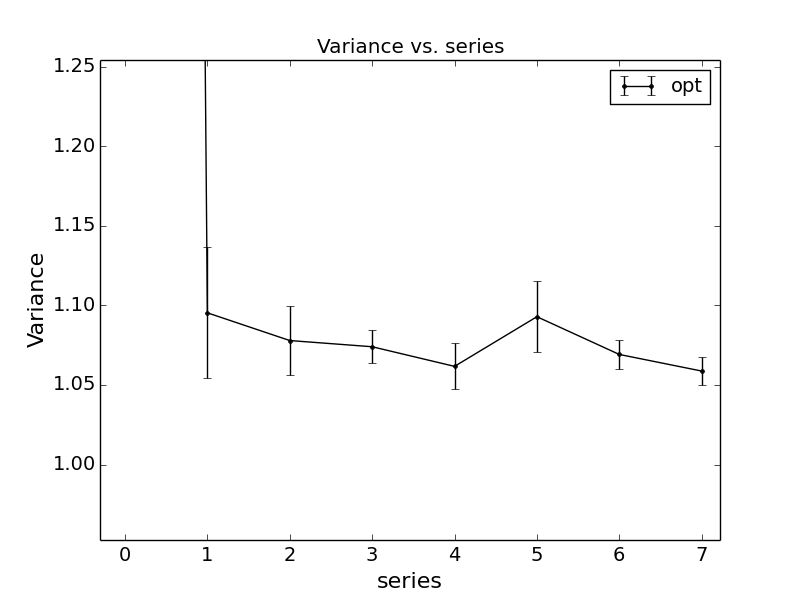
\includegraphics[trim=2mm 0mm 4mm 0mm,clip,width=0.47\textwidth]{./figures/qmca_opt_variance.png}\\
    \end{tabularx}
\fi%
  \caption{Energy and variance vs. optimization series for an 8 atom cell of diamond as plotted by \texttt{qmca}.}%
  \label{fig:qmca_opt_ev}%
\end{figure}

A good way to choose the optimal wavefunction for use in DMC is to select 
the one with lowest statistically significant energy within the set of 
optimized wavefunctions with reasonable variance (\emph{e.g.} among 
those with variance/energy ratio $<0.03$ Ha).  For pseudopotential 
calculations, minimizing according to the total energy is recommended 
to reduce locality errors in DMC.


\subsection{Judging diffusion Monte Carlo runs}
\label{sec:qmca_judge_dmc}
Judging the quality of the DMC projection process requires more 
care than this needed in VMC.  In order to reduce bias, a small 
timestep is required in the approximate projector but this also 
leads to slow equilibration and long autocorrelation times.  
Systematic errors in the projection process can also arise from 
statistical fluctuations due to pseudopotentials or from trial 
wavefunctions with larger than necessary variance.

\begin{figure}
\begin{center}
  \ifdefined\HCode  
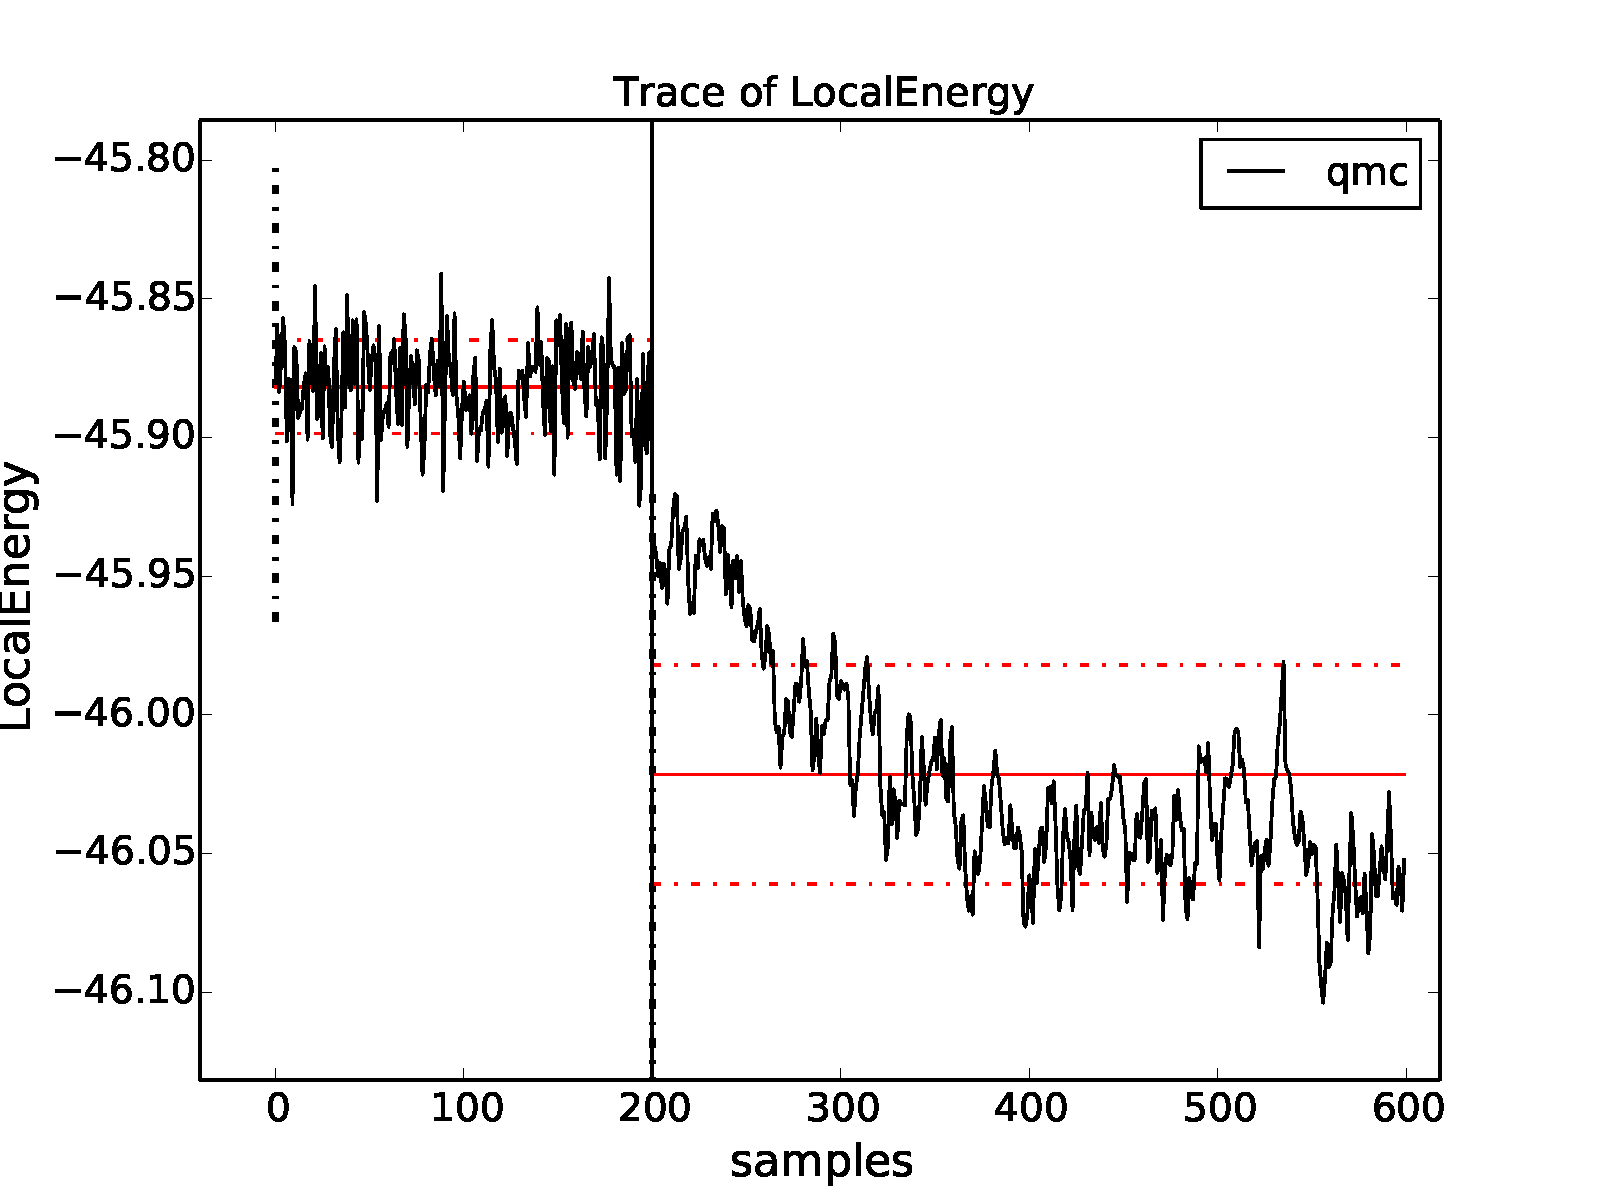
\includegraphics[trim = 0mm 0mm 0mm 0mm,clip,width=0.75\columnwidth]{./figures/qmca_short_dmc.dmn}
\else
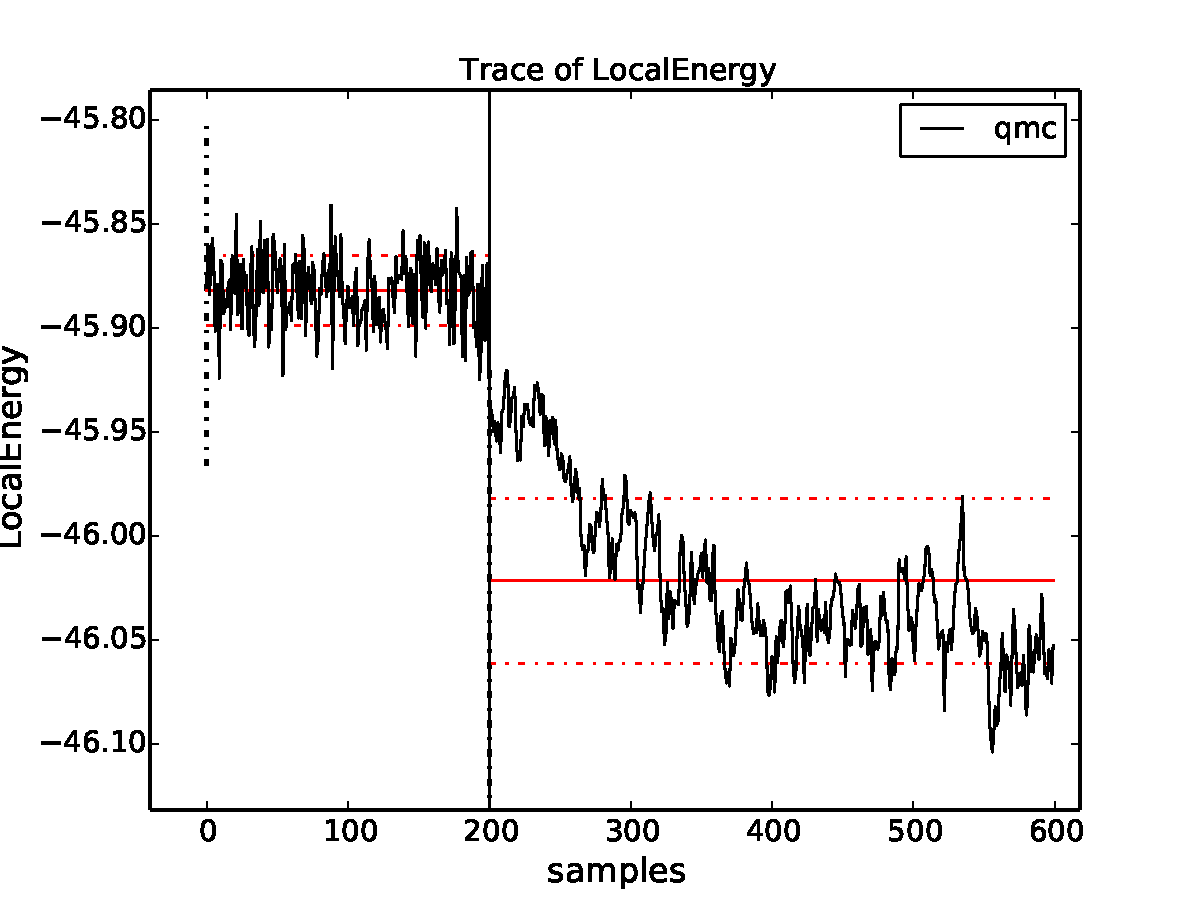
\includegraphics[trim = 0mm 0mm 0mm 0mm,clip,width=0.75\columnwidth]{./figures/qmca_short_dmc.pdf}
\fi
\end{center}
\caption{Trace of the local energy for VMC followed by DMC with a small timestep ($0.002$ Ha$^{-1}$) for an 8 atom cell of diamond generated with \texttt{qmca}.}
\label{fig:qmca_short_dmc}
\end{figure}

To illustrate the problems that can arise with respect to slow 
equilibration and long autocorrelation times, we consider the 
8 atom diamond system with VMC ($200$ blocks of $160$ steps) followed 
by DMC ($400$ blocks of $5$ steps) with a small timestep ($0.002$ Ha$^{-1}$).
A good first step in assessing the quality of any DMC run is 
to plot the trace of the local energy:
\begin{shade}
>qmca -t -q e -e 0 *scalar*
\end{shade}
\noindent
The resulting trace plot is shown in Fig. \ref{fig:qmca_short_dmc}.  
As always, the DMC local energy decreases exponentially away from 
the VMC value but in this case it takes a long time to do so.  
At least half of the DMC run is inefficiently consumed by equilibration.
If we are not careful to inspect and remove the transient, the estimated 
DMC energy will be strongly biased by the transient as shown by the 
horizontal red line (estimated mean) in the figure.  The autocorrelation 
time is also large ($\sim 12$ blocks):
\begin{shade}
>qmca -q e -e 200 --sac *s001.scalar*
qmc  series 1  LocalEnergy           =  -46.045720 +/- 0.004813   11.6
\end{shade}
\noindent
Of the included 200 blocks, fewer than 20 contribute to the estimated error 
bar, indicating that we cannot trust the reported error bar.  
This can also be demonstrated directly from the data.  If we halve the number 
of samples included to 100, we would expect from Gaussian statistics 
that the error bar would grow by a factor of $\sqrt{2}$, but instead we 
get
\begin{shade}
>qmca -q e -e 300 *s001.scalar*
qmc  series 1  LocalEnergy           =  -46.048537 +/- 0.009280
\end{shade}
\noindent
which erroneously shows an estimated increase in the error bar by a factor 
of about two.  Overall this run is simply too short to gain meaningful 
information.  

Consider the case where we are interested in the cohesive energy of 
diamond and, after having performed a timestep study of the cohesive 
energy, we have found that the energy difference between bulk diamond 
and atomic carbon converges to our required accuracy with a larger 
timestep of $0.01$ Ha$^{-1}$.  In a production setting, a small cell 
could be used to determine  the appropriate timestep while a larger 
cell would subsequently be used to obtain a converged cohesive energy, 
though for purposes of demonstration we still proceed with the 8 atom 
cell here.  The new timestep of $0.01$ Ha$^{-1}$ will result in a shorter 
autocorrelation time than the smaller timestep used previously, but 
we would like to shorten the equilibration time further still.  This 
can be achieved by using a larger timestep (say $0.02$ Ha$^{-1}$) in a 
short intermediate DMC run used to walk down the transient.  The 
rapidly achieved equilibrium with the $0.02$ Ha$^{-1}$ timestep 
projector will be much nearer to the $0.01$ Ha$^{-1}$ timestep one 
we seek than the original VMC equilibrium, and so we can expect 
a shortened secondary equilibration time in the production 
$0.01$ Ha$^{-1}$ timestep run. Note that this procedure is fully 
general, even if one has to deal with an even shorter 
timestep--\emph{e.g.} $0.002$ Ha$^{-1}$--for a particular problem.

\begin{figure}
\begin{center}
\ifdefined\HCode  
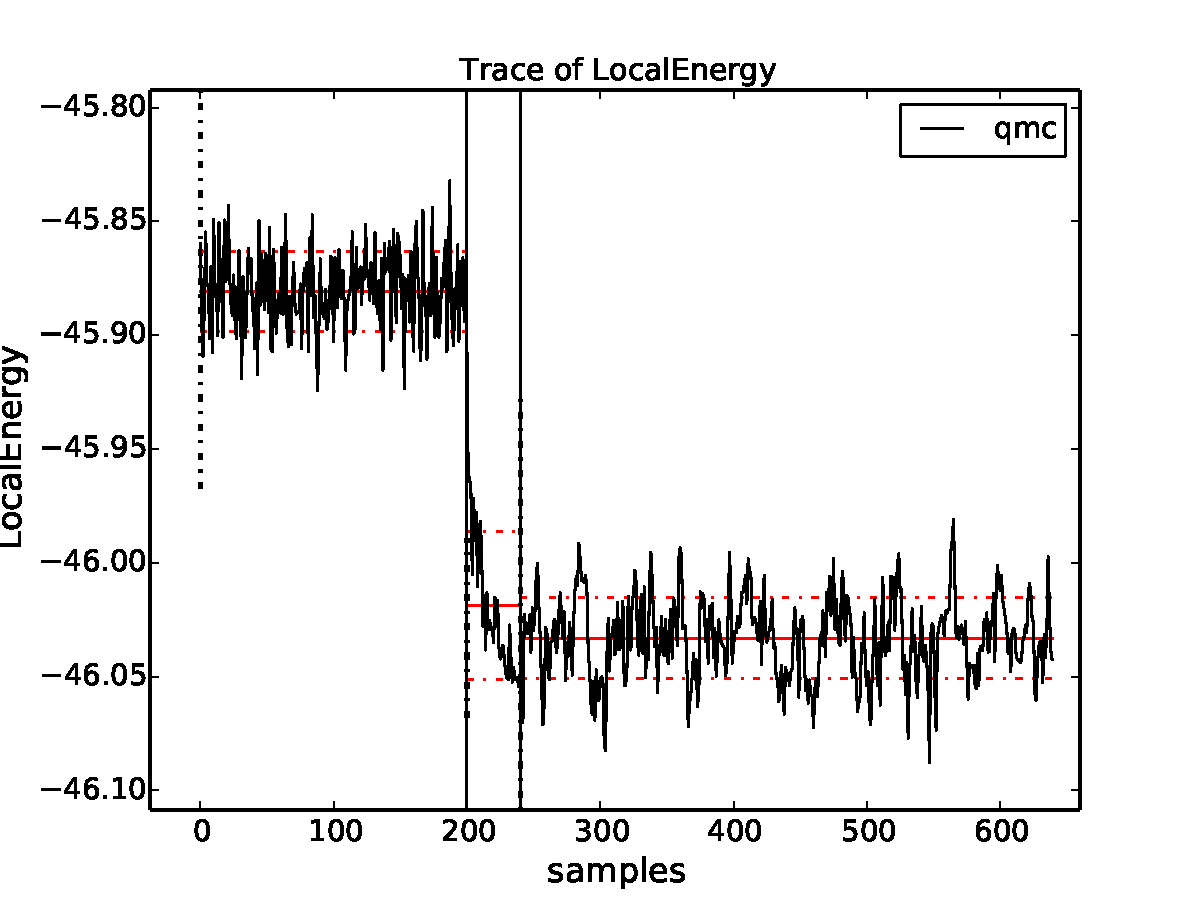
\includegraphics[trim = 0mm 0mm 0mm 0mm, clip,width=0.75\columnwidth]{./figures/qmca_accel_dmc.dmn}
\else
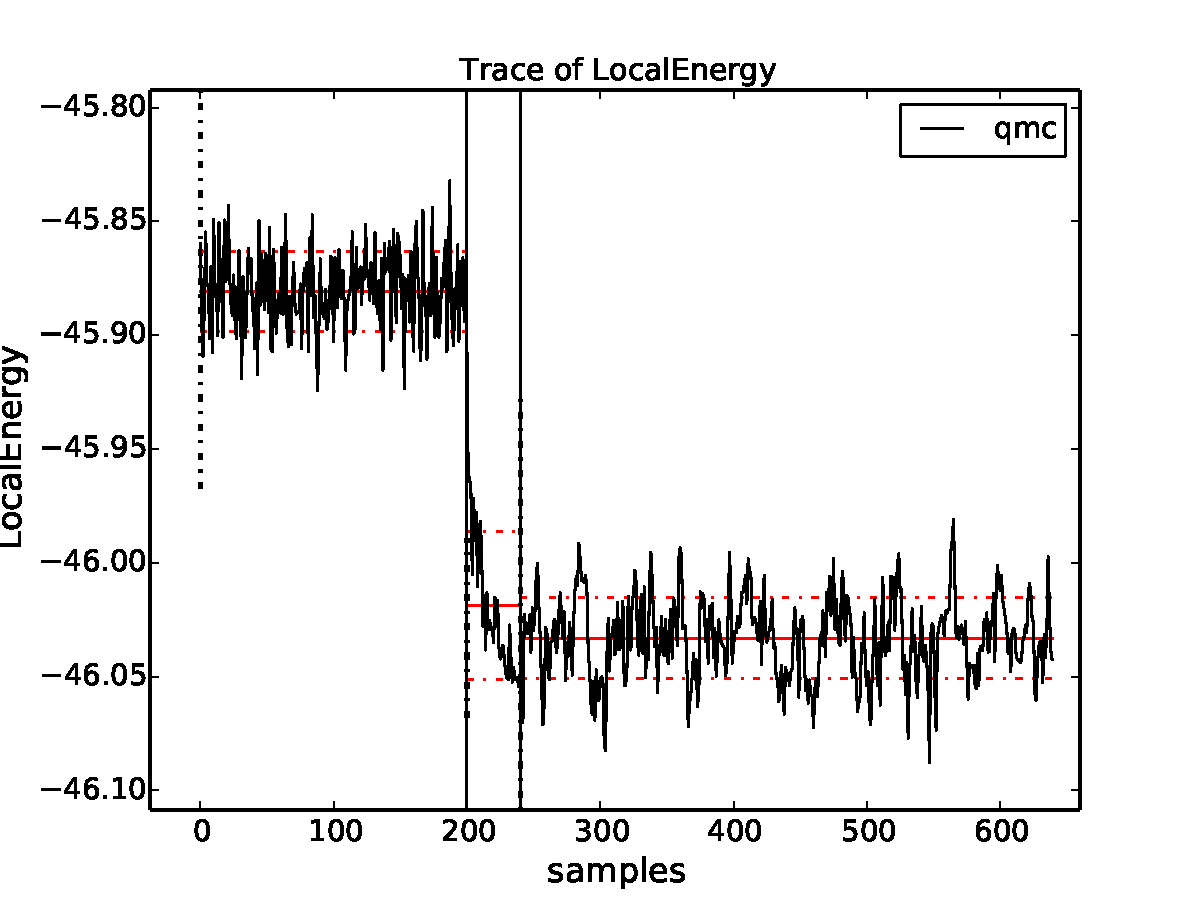
\includegraphics[trim = 0mm 0mm 0mm 0mm, clip,width=0.75\columnwidth]{./figures/qmca_accel_dmc.pdf}
\fi
\end{center}
\caption{Trace of the local energy for VMC followed by a short intermediate DMC with a large timestep ($0.02$ Ha$^{-1}$) and finally a production DMC run with a timestep of $0.01$ Ha$^{-1}$.  Calculations were performed in an 8 atom cell of diamond.} 
\label{fig:qmca_accel_dmc}
\end{figure}

We now rerun the prior example but with an intermediate DMC 
calculation using $40$ blocks of $5$ steps with a timestep of 
$0.02$ Ha$^{-1}$ followed by a production DMC calculation 
using $400$ blocks of $10$ steps with a timestep of $0.01$ Ha$^{-1}$.
We again plot the local energy trace using \texttt{qmca}
\begin{shade}
>qmca -t -q e -e 0 *scalar*
\end{shade}
\noindent
with the result shown in Fig. \ref{fig:qmca_accel_dmc}.
The projection transient has been effectively contained in the 
short DMC run with a larger timestep.  As expected, the 
production run contains only a short equilibration period.
Removing the first 20 blocks as a precaution, we obtain an estimate 
of the total energy in VMC and DMC:
\begin{shade}
>qmca -q ev -e 20 --sac qmc.*.scalar.dat 
                            LocalEnergy               Variance           ratio 
qmc  series 0  -45.881042 +/- 0.001283    1.0   1.076726 +/- 0.007013    1.0   0.0235 
qmc  series 1  -46.040814 +/- 0.005046    3.9   1.011303 +/- 0.016807    1.1   0.0220 
qmc  series 2  -46.032960 +/- 0.002077    5.2   1.014940 +/- 0.002547    1.0   0.0220 
\end{shade}
\noindent
Notice that the variance energy ratio in DMC ($0.220$ Ha) is similar to, but 
slightly smaller than, what is obtained with VMC ($0.235$ Ha).  If the DMC 
variance/energy ratio is ever significantly larger than in VMC, this is 
cause to be concerned about the correctness of the DMC run.  Also notice 
the estimated autocorrelation time ($\sim 5$ blocks).  This leaves us with 
an estimated $\sim 76$ independent samples, though we should recall that 
the autocorrelation time is also a statistical estimate which can be improved 
with more data.  We can gain a better estimate of the autocorrelation 
time by using the \texttt{*.dmc.dat} files which contain output data resolved 
per step rather than per block (there are $10\times$ more steps than blocks 
in this example case):
\begin{shade}
>qmca -q ev -e 200 --sac qmc.s002.dmc.dat 
                            LocalEnergy               Variance           ratio 
qmc  series 2  -46.032909 +/- 0.002068   31.2   1.015781 +/- 0.002536    1.4   0.0221 
\end{shade}
\noindent
This results in an estimated autocorrelation time of $\sim 31$ steps, or 
$\sim 3$ blocks, indicating that we actually have $\sim 122$ independent 
samples which should be sufficient to obtain a trustworthy error bar.
Our final DMC total energy is estimated to be $-46.0329(2)$ Ha.

\begin{figure}
\begin{center}
  \ifdefined\HCode
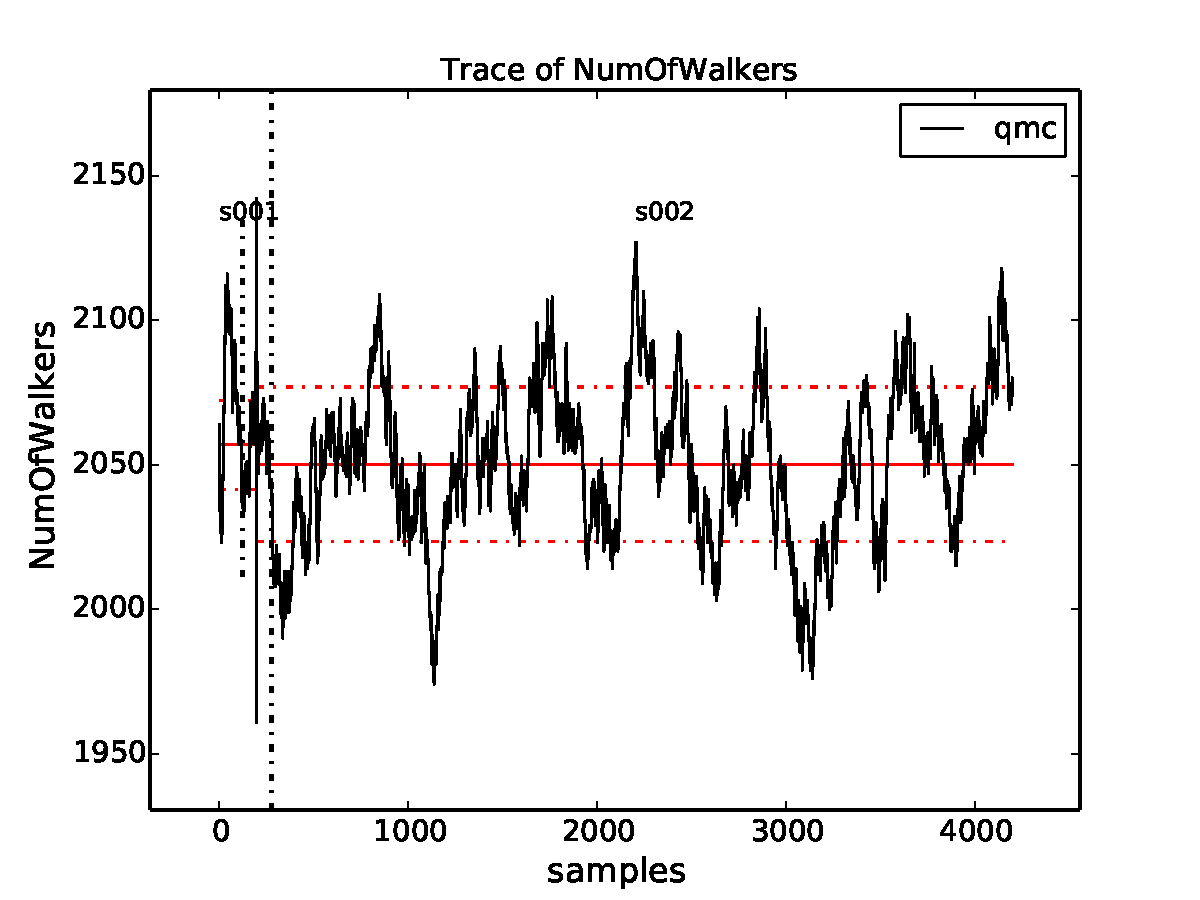
\includegraphics[trim = 0mm 0mm 0mm 0mm, clip,width=0.75\columnwidth]{./figures/qmca_pop_trace.dmn}
\else
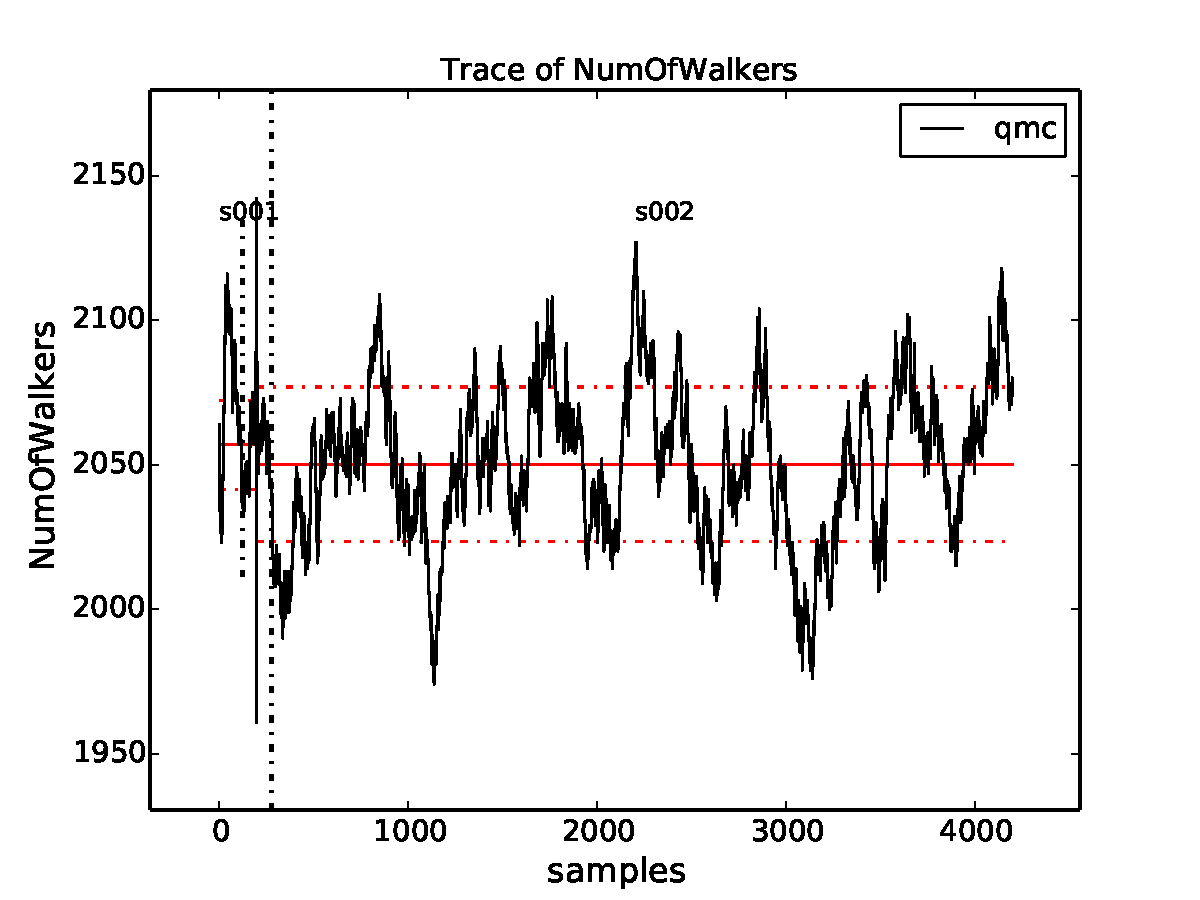
\includegraphics[trim = 0mm 0mm 0mm 0mm, clip,width=0.75\columnwidth]{./figures/qmca_pop_trace.pdf}
\fi
\end{center}
\caption{Trace of the DMC walker population for an 8 atom cell of diamond obtained with \texttt{qmca}.}
\label{fig:qmca_pop_trace}
\end{figure}

Another simulation property that should be explicitly monitored  
is the behavior of the DMC walker population.  Data regarding the 
walker population is contained in the \texttt{*.dmc.dat} files.
In Fig. \ref{fig:qmca_pop_trace} we show the trace of the DMC 
walker population for the current run:
\begin{shade}
>qmca -t -q nw *dmc.dat
qmc  series 1  NumOfWalkers          =  2056.905405 +/- 8.775527 
qmc  series 2  NumOfWalkers          =  2050.164160 +/- 4.954850 
\end{shade}
\noindent
Following a DMC run the walker population should be checked for 
two qualities: 1) that the population is sufficiently large (a number 
$>2000$ is generally sufficient to reduce population control bias) and  
2) that the population fluctuates benignly around its intended target 
value. In this case the target walker count (provided in the input file)
was $2048$ and we can confirm from the plot that the population is simply 
fluctuating around this value.  Also from the text output we have a dynamic 
population estimate of 2050(5) walkers.  Rapid population reductions or 
increases--population explosions--are indicative of problems with a run.  
These issues sometimes result from using a considerably poor wavefunction 
(see comments regarding variance/energy ratio above and in the preceding 
subsections).  QMCPACK has internal guards in place that prevent 
the population from exceeding certain maximum and minimum bounds, so 
in particularly faulty runs one might see the population ``stabilize'' 
to a constant value much larger or smaller than the target.  In these 
cases the cause(s) for the divergent population behavior need to 
be investigated and resolved before proceeding further.



\subsection{Obtaining other quantities}
\label{sec:qmca_other_quantities}
A number of other scalar valued quantities are available with 
\texttt{qmca}.  To obtain text output for all quantities 
available, simply exclude the ``\texttt{-q}'' option used in 
the prior examples.  Below is example output for a DMC calculation 
of the 8 atom diamond system from the \texttt{scalar.dat} file:
\begin{shade}
>qmca -e 20 qmc.s002.scalar.dat 
qmc  series 2 
  LocalEnergy           =          -46.0330 +/-           0.0021 
  Variance              =            1.0149 +/-           0.0025 
  Kinetic               =            33.851 +/-            0.019 
  LocalPotential        =           -79.884 +/-            0.020 
  ElecElec              =          -11.4483 +/-           0.0083 
  LocalECP              =           -22.615 +/-            0.029 
  NonLocalECP           =            5.2815 +/-           0.0079 
  IonIon                =            -51.10 +/-             0.00 
  LocalEnergy_sq        =           2120.05 +/-             0.19 
  BlockWeight           =          20514.27 +/-            48.38 
  BlockCPU              =            1.4890 +/-           0.0038 
  AcceptRatio           =         0.9963954 +/-        0.0000055 
  Efficiency            =             71.88 +/-             0.00 
  TotalTime             =            565.80 +/-             0.00 
  TotalSamples          =           7795421 +/-                0 
\end{shade}
\noindent
Similarly, for the \texttt{dmc.dat} file we get
\begin{shade}
>qmca -e 20 qmc.s002.dmc.dat 
qmc  series 2 
  LocalEnergy           =          -46.0329 +/-           0.0020 
  Variance              =            1.0162 +/-           0.0025 
  TotalSamples          =           8201275 +/-                0 
  TrialEnergy           =          -46.0343 +/-           0.0023 
  DiffEff               =         0.9939150 +/-        0.0000088 
  Weight                =           2050.23 +/-             4.82 
  NumOfWalkers          =              2050 +/-                5 
  LivingFraction        =          0.996427 +/-         0.000021 
  AvgSentWalkers        =            0.2625 +/-           0.0011 
\end{shade}

Any subset of desired quantities can be obtained by using the 
``\texttt{-q}'' option with either the full names of the quantities 
listed above 
\begin{shade}
>qmca -q 'LocalEnergy Kinetic LocalPotential' -e 20 qmc.s002.scalar.dat 
qmc  series 2 
  LocalEnergy           =          -46.0330 +/-           0.0021 
  Kinetic               =            33.851 +/-            0.019 
  LocalPotential        =           -79.884 +/-            0.020 
\end{shade}
\noindent
or with their corresponding abbreviations
\begin{shade}
>qmca -q ekp -e 20 qmc.s002.scalar.dat 
qmc  series 2 
  LocalEnergy           =          -46.0330 +/-           0.0021 
  Kinetic               =            33.851 +/-            0.019 
  LocalPotential        =           -79.884 +/-            0.020 
\end{shade}
\noindent
Abbreviations for each quantity can be found by typing \texttt{qmca}
at the command line with no other input.  A current list is provided 
below:
\begin{shade}
  Abbreviations and full names for quantities:
    ar              = AcceptRatio
    bc              = BlockCPU
    bw              = BlockWeight
    ce              = CorrectedEnergy
    de              = DiffEff
    e               = LocalEnergy
    ee              = ElecElec
    eff             = Efficiency
    ii              = IonIon
    k               = Kinetic
    kc              = KEcorr
    l               = LocalECP
    le2             = LocalEnergy_sq
    mpc             = MPC
    n               = NonLocalECP
    nw              = NumOfWalkers
    p               = LocalPotential
    sw              = AvgSentWalkers
    te              = TrialEnergy
    ts              = TotalSamples
    tt              = TotalTime
    v               = Variance
    w               = Weight
\end{shade}
\noindent
Please see the output overview for \texttt{scalar.dat} 
(Sec. \ref{sec:scalardat_file}) and \texttt{dmc.dat} 
(Sec. \ref{sec:dmc_file}) for more information about 
these quantities.  The data analysis aspects for these 
quantities is essentially the same as for the local 
energy as covered in the preceding subsections. 
Quantities that do not belong to an equilibrium distribution 
(\emph{e.g.} \texttt{BlockCPU}) are somewhat different, though they 
still exhibit statistical fluctuations.


\subsection{Processing multiple files}
\label{sec:qmca_multiple_files}
Batch file processing is a common use case for \texttt{qmca}. 
If we consider an ``equation of state'' calculation involving 
the 8 atom diamond cell we have used so far, we might be interested 
in the total energy for the various supercell volumes along the 
trajectory from compression to expansion.  After checking 
the traces (``\texttt{qmca -t -q e scale\_*/vmc/*scalar*}'') 
to settle on a sensible equilibration cutoff as discussed in 
the preceding subsections we can obtain the total energies 
all at once:
\begin{shade}
>qmca -q ev -e 40 scale_*/vmc/*scalar*
                            LocalEnergy               Variance           ratio 
scale_0.80/vmc/qmc  series 0 -44.670984 +/- 0.006051  2.542384 +/- 0.019902  0.0569 
scale_0.82/vmc/qmc  series 0 -44.982818 +/- 0.005757  2.413011 +/- 0.022626  0.0536 
scale_0.84/vmc/qmc  series 0 -45.228257 +/- 0.005374  2.258577 +/- 0.019322  0.0499 
scale_0.86/vmc/qmc  series 0 -45.415842 +/- 0.005532  2.204980 +/- 0.052978  0.0486 
scale_0.88/vmc/qmc  series 0 -45.570215 +/- 0.004651  2.061374 +/- 0.014359  0.0452 
scale_0.90/vmc/qmc  series 0 -45.683684 +/- 0.005009  1.988539 +/- 0.018267  0.0435 
scale_0.92/vmc/qmc  series 0 -45.751359 +/- 0.004928  1.913282 +/- 0.013998  0.0418 
scale_0.94/vmc/qmc  series 0 -45.791622 +/- 0.005026  1.843704 +/- 0.014460  0.0403 
scale_0.96/vmc/qmc  series 0 -45.809256 +/- 0.005053  1.829103 +/- 0.014536  0.0399 
scale_0.98/vmc/qmc  series 0 -45.806235 +/- 0.004963  1.775391 +/- 0.015199  0.0388 
scale_1.00/vmc/qmc  series 0 -45.783481 +/- 0.005293  1.726869 +/- 0.012001  0.0377 
scale_1.02/vmc/qmc  series 0 -45.741655 +/- 0.005627  1.681776 +/- 0.011496  0.0368 
scale_1.04/vmc/qmc  series 0 -45.685101 +/- 0.005353  1.682608 +/- 0.015423  0.0368 
scale_1.06/vmc/qmc  series 0 -45.615164 +/- 0.005978  1.652155 +/- 0.010945  0.0362 
scale_1.08/vmc/qmc  series 0 -45.543037 +/- 0.005191  1.646375 +/- 0.013446  0.0361 
scale_1.10/vmc/qmc  series 0 -45.450976 +/- 0.004794  1.707649 +/- 0.048186  0.0376 
scale_1.12/vmc/qmc  series 0 -45.371851 +/- 0.005103  1.686997 +/- 0.035920  0.0372 
scale_1.14/vmc/qmc  series 0 -45.265490 +/- 0.005311  1.631614 +/- 0.012381  0.0360 
scale_1.16/vmc/qmc  series 0 -45.161961 +/- 0.004868  1.656586 +/- 0.014788  0.0367 
scale_1.18/vmc/qmc  series 0 -45.062579 +/- 0.005971  1.671998 +/- 0.019942  0.0371 
scale_1.20/vmc/qmc  series 0 -44.960477 +/- 0.004888  1.651864 +/- 0.009756  0.0367 
\end{shade}
\noindent

In this case, we are using a Jastrow factor optimized only at the 
equilibrium geometry (``\texttt{scale\_1.00}'') but with radial 
cutoffs restricted to the Wigner-Seitz radius of the most compressed 
supercell (``\texttt{scale\_0.80}'') to avoid introducing wavefunction 
cusps at the cell boundary (QMCPACK would have aborted with a warning in 
this case, had we tried).  It is clear that this restricted Jastrow factor 
is not an optimal choice as it yields variance/energy ratios between $0.036$ 
and $0.057$ Ha.  This issue is largely a result of our undersized (8 atom) 
supercell and larger cells should always be used in real production 
calculations.

Batch processing is also possible for multiple quantities.  If multiple 
quantities are requested, an additional line is inserted to separate 
results from different runs:
\begin{shade}
>qmca -q 'e bc eff' -e 40 scale_*/vmc/*scalar*
scale_0.80/vmc/qmc  series 0 
  LocalEnergy           =          -44.6710 +/-           0.0061 
  BlockCPU              =           0.02986 +/-          0.00038 
  Efficiency            =          38104.00 +/-             0.00 

scale_0.82/vmc/qmc  series 0 
  LocalEnergy           =          -44.9828 +/-           0.0058 
  BlockCPU              =           0.02826 +/-          0.00013 
  Efficiency            =          44483.91 +/-             0.00 

scale_0.84/vmc/qmc  series 0 
  LocalEnergy           =          -45.2283 +/-           0.0054 
  BlockCPU              =           0.02747 +/-          0.00030 
  Efficiency            =          52525.12 +/-             0.00 

scale_0.86/vmc/qmc  series 0 
  LocalEnergy           =          -45.4158 +/-           0.0055 
  BlockCPU              =           0.02679 +/-          0.00013 
  Efficiency            =          50811.55 +/-             0.00 

scale_0.88/vmc/qmc  series 0 
  LocalEnergy           =          -45.5702 +/-           0.0047 
  BlockCPU              =           0.02598 +/-          0.00015 
  Efficiency            =          74148.79 +/-             0.00 

scale_0.90/vmc/qmc  series 0 
  LocalEnergy           =          -45.6837 +/-           0.0050 
  BlockCPU              =           0.02527 +/-          0.00011 
  Efficiency            =          65714.98 +/-             0.00 

...
\end{shade}



\subsection{Twist averaging}
\label{sec:qmca_twist_average}
Twist averaging can be performed straightforwardly for any 
output quantity listed in Sec. \ref{sec:qmca_other_quantities} 
with \texttt{qmca}.  We illustrate these capabilities by 
repeating the 8 atom diamond DMC runs performed in Sec. 
\ref{sec:qmca_judge_dmc} at eight real valued supercell twist 
angles (a $2\times 2\times 2$ Monkhorst-Pack grid centered at 
the $\Gamma$-point).  Data traces for each twist can be overlapped 
on the same plot:
\begin{shade}
>qmca -to -q e -e '30 20 30' *scalar* --legend outside
\end{shade}
\noindent
The ``\texttt{-o}'' option requests the plots be overlapped; 
eight separate plots would be generated otherwise.  The 
equilibration input ``\texttt{-e '30 20 30'}'' cuts out from 
the analyzed data the first 30 blocks for series 0 (VMC), 
20 blocks for series 1 (intermediate DMC), and 30 blocks for 
series 2 (production DMC).  The resulting plot is shown in 
Fig. \ref{fig:qmca_twist_overlap}

\begin{figure}
\begin{center}
\ifdefined\HCode
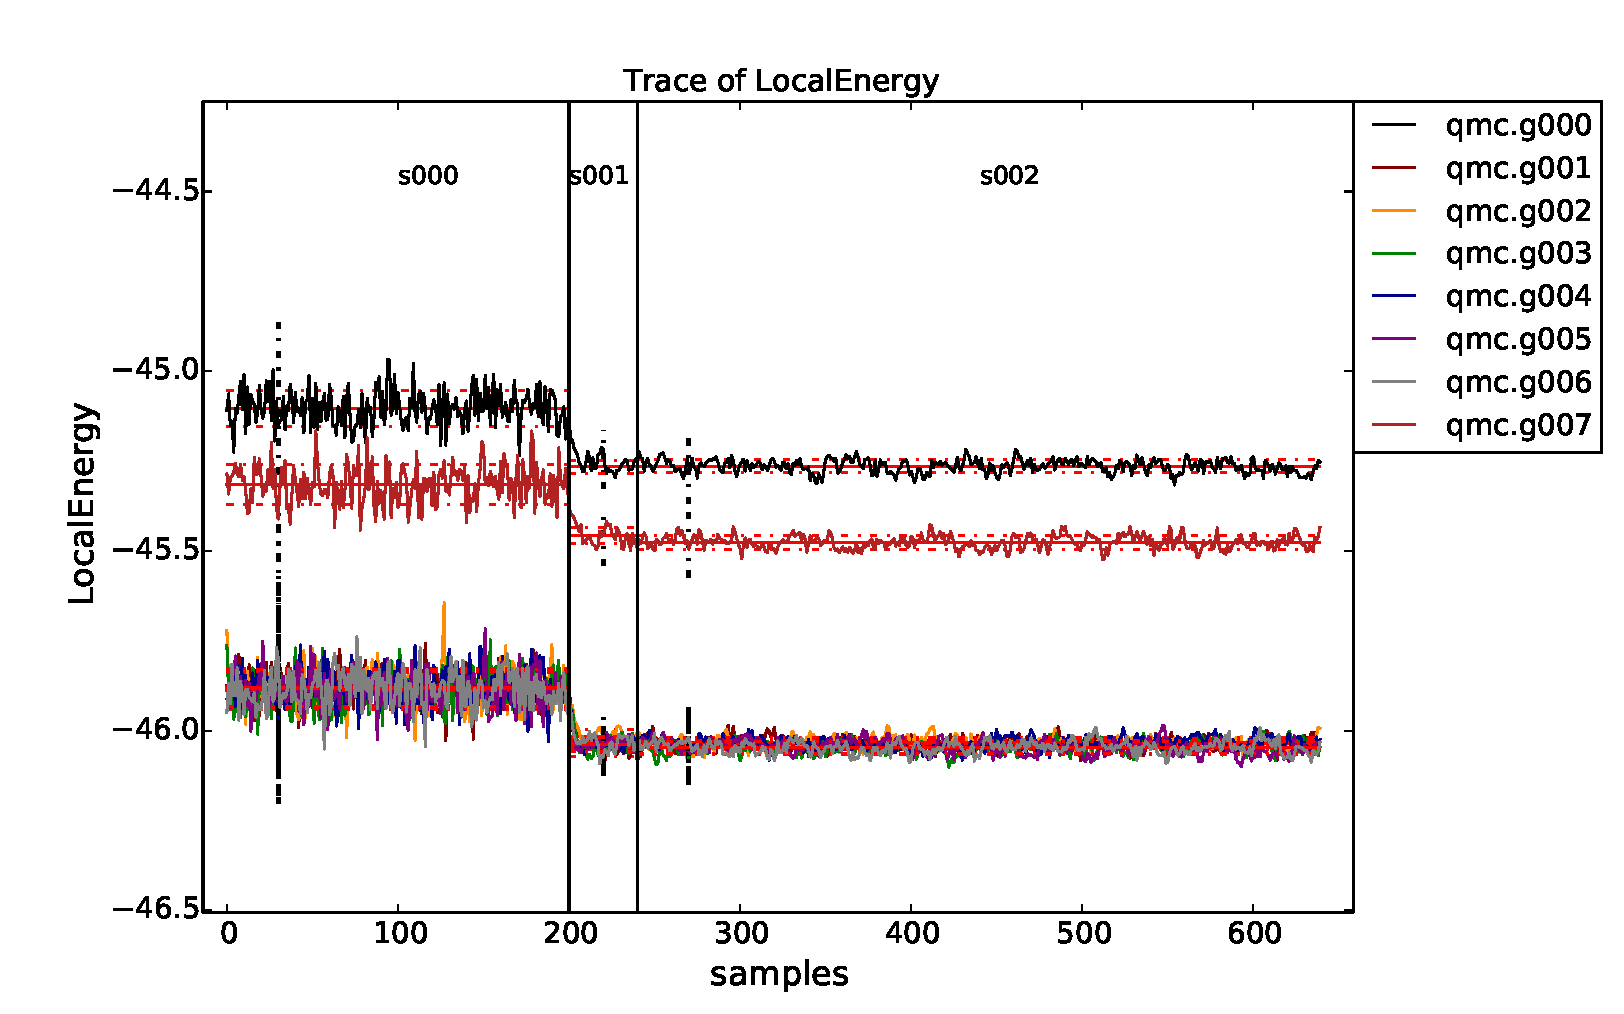
\includegraphics[trim = 0mm 0mm 0mm 0mm, clip,width=0.9\columnwidth]{./figures/qmca_twist_trace_overlap.dmn}
\else
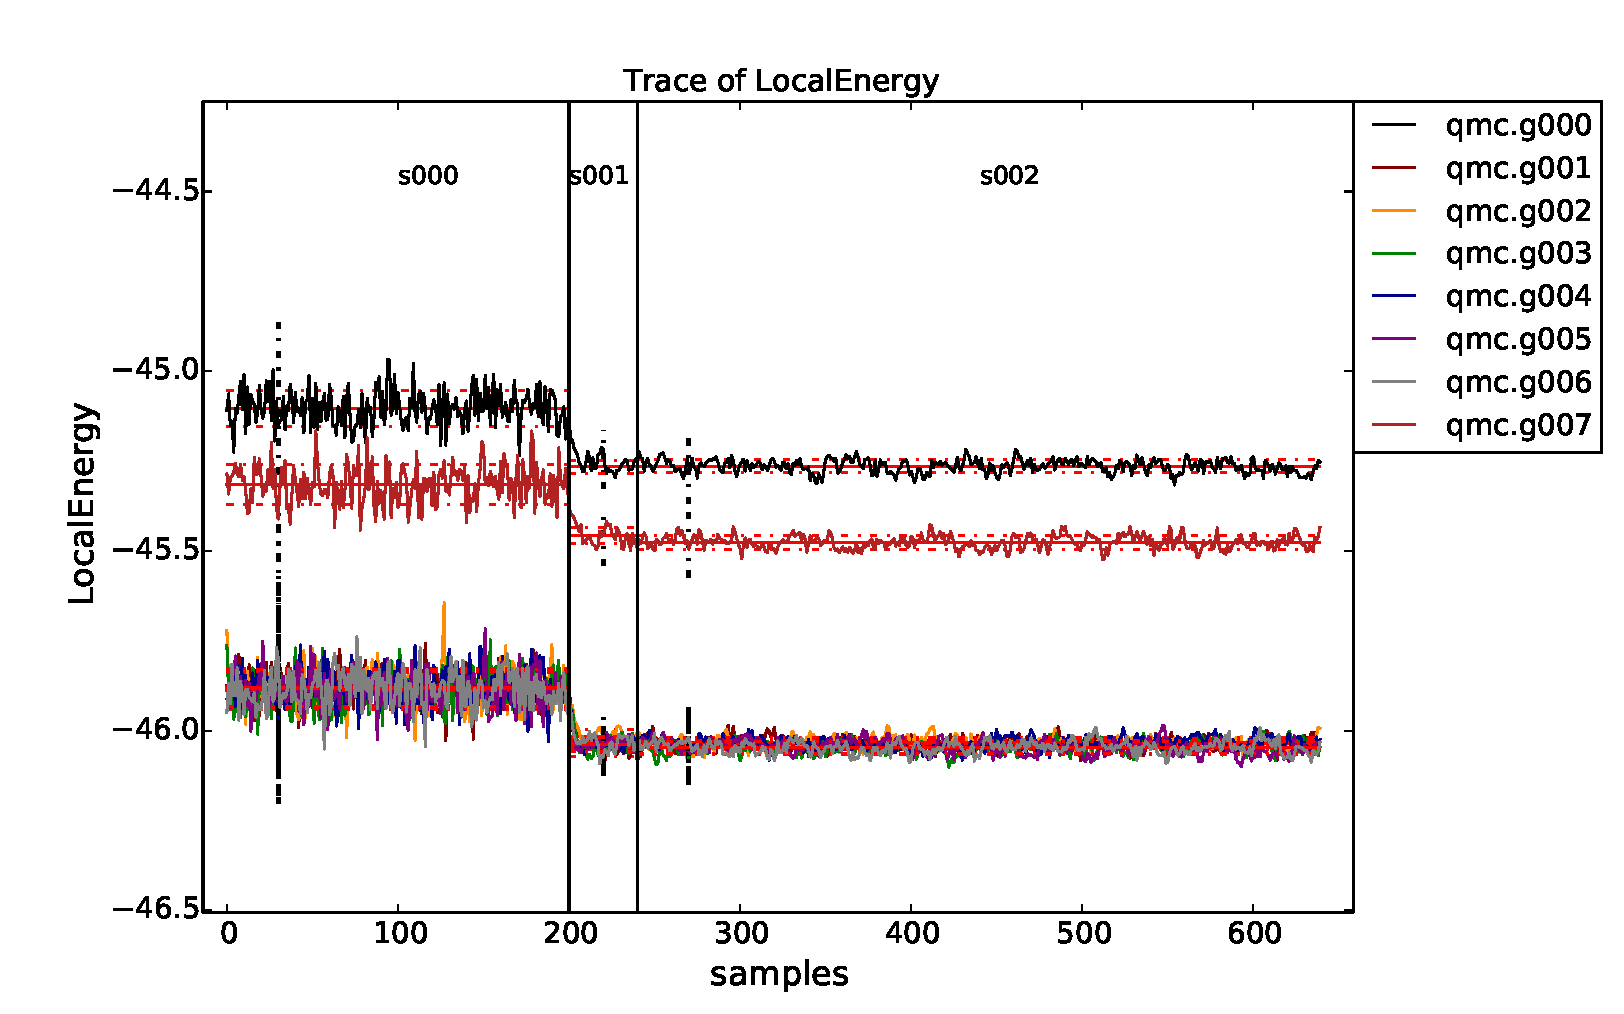
\includegraphics[trim = 0mm 0mm 0mm 0mm, clip,width=0.9\columnwidth]{./figures/qmca_twist_trace_overlap.pdf}
\fi
\end{center}
\caption{Overlapped energy traces from VMC to DMC for an 8 supercell of diamond obtained with \texttt{qmca}.  Data for each twist appears in a different color.}
\label{fig:qmca_twist_overlap}
\end{figure}

Twist averaging is performed by providing the ``\texttt{-a}'' 
option.  If provided on its own, uniform weights are applied 
to each twist angle.  To obtain a trace plot with twist averaging 
enforced, use a command similar to the following:
\begin{shade}
>qmca -a -t -q e -e '30 20 30' *scalar*
\end{shade}
\noindent
The resulting plot is shown in Fig. \ref{fig:qmca_twist_average}.
As can be seen from the trace plot, the chosen equilibration lengths 
are appropriate and we proceed to obtain the twist averaged total energy
from the \texttt{scalar.dat} files
\begin{shade}
>qmca -a -q ev -e 30 --sac *s002.scalar*
                            LocalEnergy               Variance           ratio 
avg  series 2  -45.873369 +/- 0.000753    5.3   1.028751 +/- 0.001056    1.3   0.0224 
\end{shade}
\noindent
and also from the \texttt{dmc.dat} files
\begin{shade}
>qmca -a -q ev -e 300 --sac *s002.dmc*
                            LocalEnergy               Variance           ratio 
avg  series 2  -45.873371 +/- 0.000741   30.5   1.028843 +/- 0.000972    1.6   0.0224 
\end{shade}
\noindent
yielding a twist averaged total energy of $-45.8733(8)$ Ha. 

\begin{figure}
\begin{center}
\ifdefined\HCode
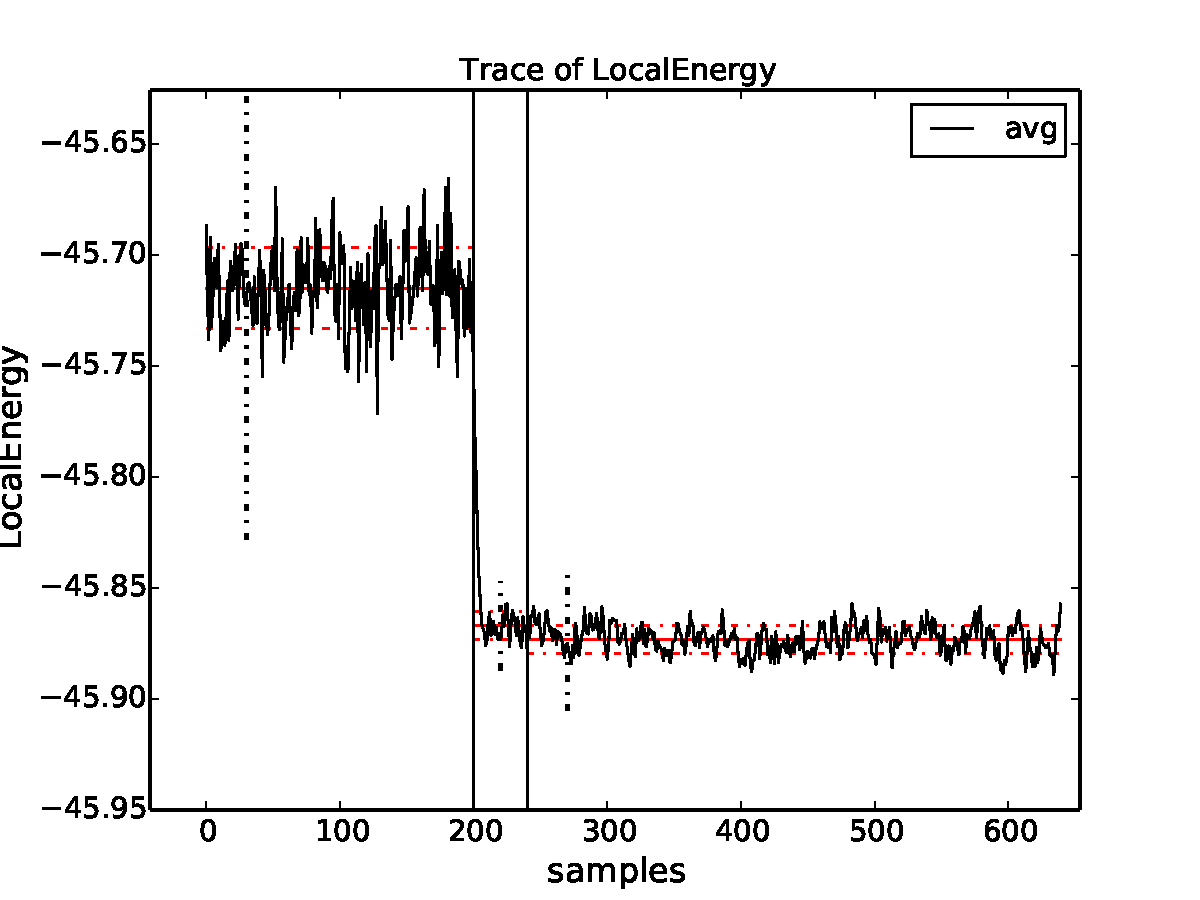
\includegraphics[trim = 0mm 0mm 0mm 0mm, clip,width=0.75\columnwidth]{./figures/qmca_twist_average_trace.dmn}
\else
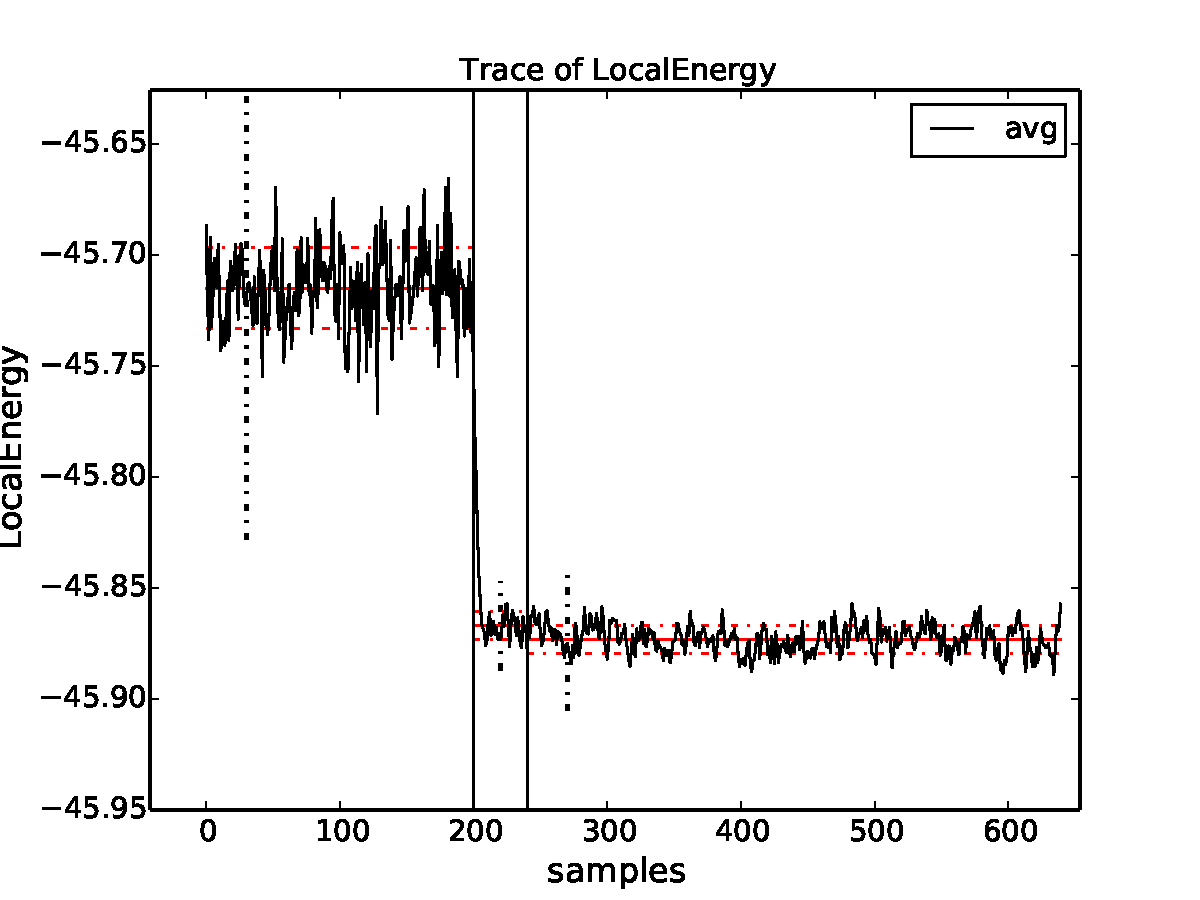
\includegraphics[trim = 0mm 0mm 0mm 0mm, clip,width=0.75\columnwidth]{./figures/qmca_twist_average_trace.pdf}
\fi
\end{center}
\caption{Twist averaged energy trace from VMC to DMC for an 8 supercell of diamond obtained with \texttt{qmca}.}
\label{fig:qmca_twist_average}
\end{figure}

As can be seen from the Fig. \ref{fig:qmca_twist_overlap}, some of the twist 
angles are degenerate. This is seen more clearly in the text output:
\begin{shade}
>qmca -q ev -e 30 *s002.scalar*
                            LocalEnergy               Variance           ratio 
qmc.g000  series 2  -45.264510 +/- 0.001942   1.057065 +/- 0.002318   0.0234 
qmc.g001  series 2  -46.035511 +/- 0.001806   1.015992 +/- 0.002836   0.0221 
qmc.g002  series 2  -46.035410 +/- 0.001538   1.015039 +/- 0.002661   0.0220 
qmc.g003  series 2  -46.047285 +/- 0.001898   1.018219 +/- 0.002588   0.0221 
qmc.g004  series 2  -46.034225 +/- 0.002539   1.013420 +/- 0.002835   0.0220 
qmc.g005  series 2  -46.046731 +/- 0.002963   1.018337 +/- 0.004109   0.0221 
qmc.g006  series 2  -46.047133 +/- 0.001958   1.021483 +/- 0.003082   0.0222 
qmc.g007  series 2  -45.476146 +/- 0.002065   1.070456 +/- 0.003133   0.0235 
\end{shade}
\noindent
The degenerate twists grouped by set are $\{0\}$, $\{1,2,4\}$, $\{3,5,6\}$, 
$\{7\}$.

Alternatively, the run could have been performed at \emph{only} the four 
unique (irreducible) twist angles.  We will emulate this situation by 
analyzing data for twists 0, 1, 3, and 7 only.  In a production setting 
with irreducibly weighted twists, run would be performed on these twists 
alone; we reuse the uniform twist data for illustration purposes only.  

We can use \texttt{qmca} to perform twist averaging with different 
weights applied to each twist
\begin{shade}
>qmca -a -w '1 3 3 1' -q ev -e 30 *g000*2*sc* *g001*2*sc* *g003*2*sc* *g007*2*sc*
                            LocalEnergy               Variance           ratio 
avg  series 2  -45.873631 +/- 0.001044   1.028769 +/- 0.001520   0.0224 
\end{shade}
\noindent
yielding a total energy value of $-45.874(1)$ Ha, in agreement with the 
uniform weighted twist average performed above.  

The decision of whether or not to perform irreducible weighted twist 
averaging should be made on the basis of efficiency.  The relative 
efficiency of irreducible vs. uniform weighted twist averaging 
depends on the irreducible weights and the ratio of the lengths of 
the available sampling and equilibration periods.  A formula for 
the relative efficiency of these two cases is derived and discussed 
in more detail in Appendix \ref{sec:app_ta_efficiency}.


\subsection{Setting output units}
\label{sec:qmca_output_units}
Estimates outputted by \texttt{qmca} are in Hartree units by 
default.  The output units for energetic quantities can be 
changed by using the ``\texttt{-u}'' option.  

\vspace{3mm}
\noindent
Energy in Hartrees:
\begin{shade}
>qmca -q e -u Ha -e 20 qmc.s002.scalar.dat
qmc  series 2  LocalEnergy           =  -46.032960 +/- 0.002077
\end{shade}

\noindent
Energy in electron volts:
\begin{shade}
>qmca -q e -u eV -e 20 qmc.s002.scalar.dat
qmc  series 2  LocalEnergy           =  -1252.620565 +/- 0.056521 
\end{shade}

\noindent
Energy in Rydbergs:
\begin{shade}
>qmca -q e -u rydberg -e 20 qmc.s002.scalar.dat
qmc  series 2  LocalEnergy           =  -92.065919 +/- 0.004154   
\end{shade}

\noindent
Energy in kilojoules per mole:
\begin{shade}
>qmca -q e -u kj_mol -e 20 qmc.s002.scalar.dat
qmc  series 2  LocalEnergy           =  -120859.512998 +/- 5.453431   
\end{shade}


\subsection{Speeding up trace plotting}
\label{sec:qmca_fast_trace_plot}
When working with many files or files with many entries, 
\texttt{qmca} may take a long time to produce plots.  The time 
delay is actually due to the autocorrelation time estimate 
used to calculate error bars.  The calculation time for 
the autocorrelation scales as $\mathcal{O}(M^2)$, with $M$ being 
the number of statistical samples.  If you are only interested 
in plotting traces and not in the estimated error bars, the 
autocorrelation time estimation can be turned off with the 
``\texttt{--noac}'' option:
\begin{shade}
>qmca -t -q e -e 20 --noac qmc.s002.scalar.dat
\end{shade}
\noindent
Please note that the resulting error bars printed to the console 
will be underestimated and are not meaningful.  Do \emph{not} 
use ``\texttt{--noac}'' in conjunction with the ``\texttt{-p}'' 
plotting option as these plots are of no use without meaningful 
error bars.


\subsection{Short usage examples}
\label{sec:qmca_short_examples}
\noindent
Plotting a trace of the local energy:
\begin{shade}
>qmca -t -q e *scalar*
\end{shade}
\noindent
Applying an equilibration cutoff to VMC data (series 0):
\begin{shade}
>qmca -q e -e 30 *s000.scalar*
\end{shade}
\noindent
Applying the same equilibration cutoff to VMC and DMC data (series 0, 1, 2):
\begin{shade}
>qmca -q e -e 20 *scalar*
\end{shade}
\noindent
Applying different equilibration cutoffs to VMC and DMC data (series 0, 1, 2):
\begin{shade}
>qmca -q e -e '30 20 40' *scalar*
\end{shade}
\noindent
Obtaining the energy, variance, and variance/energy ratio for all series:
\begin{shade}
>qmca -q ev -e 30 *scalar*
\end{shade}
\noindent
Overlaying plots of mean + error bar for energy and variance for separate 
two- and three- body Jastrow optimization runs:
\begin{shade}
>qmca -po -q ev ./optJ2/*scalar* ./optJ3/*scalar*
\end{shade}
\noindent
Obtaining the acceptance ratio:
\begin{shade}
>qmca -q ar -e 30 *scalar*
\end{shade}
\noindent
Obtaining the average DMC walker population:
\begin{shade}
>qmca -q nw -e 400 *s002.dmc.dat
\end{shade}
\noindent
Obtaining the Monte Carlo efficiency:
\begin{shade}
>qmca -q eff -e 30 *scalar*
\end{shade}
\noindent
Obtaining the total wallclock time per series:
\begin{shade}
>qmca -q tt -e 0 *scalar*
\end{shade}
\noindent
Obtaining the average wallclock time spent per block:
\begin{shade}
>qmca -q bc -e 0 *scalar*
\end{shade}
\noindent
Obtaining a subset of desired quantities:
\begin{shade}
>qmca -q 'e v ar eff' -e 30 *scalar*
\end{shade}
\noindent
Obtaining all available quantities:
\begin{shade}
>qmca -e 30 *scalar*
\end{shade}
\noindent
Obtaining the twist averaged total energy with uniform weights:
\begin{shade}
>qmca -a -q e -e 40 *g*s002.scalar.dat
\end{shade}
\noindent
Obtaining the twist averaged total energy with specific weights:
\begin{shade}
>qmca -a -w '1 3 3 1' -q e -e 40 *g*s002.scalar.dat
\end{shade}
\noindent
Obtaining the local, kinetic, and potential energies in eV:
\begin{shade}
>qmca -q ekp -e 30 -u eV *scalar*
\end{shade}



\subsection{Production quality checklist}
\label{sec:qmca_production_checklist}

\begin{enumerate}
  \item{Inspect the trace plots (``\texttt{-t}'' option) for any 
    oddities in the data.  Typical behavior is a short equilibration 
    period followed by benign fluctuations around a clear mean value.  
    There should not be any large spikes in the data. This applies 
    to \emph{all} runs (VMC, optimization, DMC, etc.).}

  \item{Remove all equilibration steps (``\texttt{-e}'' option) from 
    the data by inspecting the trace plot.}

  \item{Check the quality of the orbitals (standalone Jastrow-less 
    VMC or sometimes the first \texttt{scalar} file produced during 
    optimization) by inspecting the variance/energy ratio 
    ``\texttt{qmca -q ev *scalar*}''.  For pseudopotential systems 
    without a Jastrow, the variance/energy ratio should not exceed 
    $0.2$ Ha, otherwise there is a problem with the orbitals.}

  \item{Check the quality of the optimized Jastrow factor by inspecting 
    the variance/energy ratio.  For pseudopotential systems with a 
    Jastrow, the variance/energy ratio should not exceed $0.04$ Ha 
    for pseudopotential systems.  A good Jastrow is indicated by a 
    variance/energy ratio in the range $0.01-0.03$ Ha.  A value less 
    than $0.01$ Ha is difficult to achieve.}

  \item{Confirm that the optimization has converged by plotting the 
    energy and variance vs. optimization series 
    (``\texttt{qmca -p -q ev *scalar*}'').  Do not assume that 
    optimization has converged in only a few cycles.  Use at least 
    10 cycles of with around 100,000 samples unless you already have 
    experience with the system in question.}

  \item{Optimize Jastrow factors according to energy minimization to 
    reduce locality errors arising from the use of non-local 
    pseudopotentials in DMC.  A good approach is to optimize with a 
    few cycles of variance minimization followed by several cycles of 
    energy minimization.}

  \item{Occasionally try optimizing with more samples and/or cycles 
    to see if improved results are obtained.}

  \item{If using a B-spline representation of the orbitals, converge 
    the VMC energy and variance with respect to the mesh size (controlled 
    via meshfactor).  This is best done in the presence of any 
    Jastrow factor to reduce noise.  Consider using the hybrid LMTO 
    representation of the orbitals as this can reduce both the VMC/DMC 
    variance and DMC timestep error in addition to saving memory.}

  \item{Check the variance/energy ratio of all production VMC and DMC 
    calculations.  In all cases the DMC ratio should be slightly 
    less than the VMC one and both should abide the guidelines above, 
    \emph{i.e.} the ratio should be less than $0.04$ Ha for 
    pseudopotential systems.  The production ratio should also be 
    consistent with what is observed during wavefunction optimization.}

  \item{Be aware of population control bias in DMC.  Run with a 
    population of $\sim 2000$ or greater.  Occasionally repeat a run 
    using a larger population to explicitly confirm that population 
    control bias is small.}

  \item{Check the stability of the DMC walker population by plotting 
    the trace of the population size (``\texttt{qmca -t -q nw *dmc.dat}'').  
    Verify that the average walker population is consistent with 
    the requested value provided in the input.}

  \item{In DMC, perform a timestep study to either 1) obtain 
    extrapolated results, or 2) obtain a timestep for future 
    production where an energy difference shows convergence 
    (\emph{e.g.} a band gap or defect formation energy).  For 
    pseudopotential systems, converged timesteps for many systems 
    are in the range $0.002-0.01$ Ha$^{-1}$, but the actual converged 
    timestep must be explicitly checked.}

  \item{In periodic systems, converge the total energy with respect to 
    the size of the twist/k-point grid.  Results for smaller systems 
    can easily be transferred to larger ones (\emph{e.g.} a 2x2x2 twist 
    grid in a 2x2x2 tiled cell is equivalent to a 1x1x1 twist grid in a 
    4x4x4 tiled cell)}.

  \item{In periodic systems, perform finite size extrapolation 
    including two body corrections (needed for cohesive energy/phase 
    stability studies) unless it can be shown that finite size effects 
    cancel for the energy difference in question (\emph{e.g.} some 
    defect formation energies).}

\end{enumerate}


\section{Using the qmc-fit tool for statistical timestep extrapolation and curve fitting}
\label{sec:qmcfit}

The \texttt{qmc-fit} tool is used to provide statistical estimates of
curve fitting parameters based on QMCPACK data.  While \texttt{qmc-fit}
will eventually support many types of fitted curves (\emph{e.g.} Morse
potential binding curves, various equation of state fitting curves, etc.),
it is currently limited to estimating fitting parameters related to
timestep extrapolation.

\subsection{The jack-knife statistical technique}
The \texttt{qmc-fit} tool obtains estimates of fitting parameter
means and associated error bars via the ``jack-knife''
technique.  The jack-knife method is a powerful and general tool
to obtain meaningful error bars for any quantity that is related
in a non-linear fashion to an underlying set of statistical data.
For this reason, we give a brief overview of the jack-knife
technique before proceeding with usage instructions for the
\texttt{qmc-fit} tool.

Consider $N$ statistical variables $\{x_n\}_{n=1}^N$ that have
been outputted by one or more simulation runs.  If we have
$M$ samples of each of the $N$ variables, then the mean values
of each these variables can be estimated in the standard way,
i.e. $\bar{x}_n\approx \tfrac{1}{M}\sum_{m=1}^Mx_{nm}$.

Suppose we are interested in $P$ statistical quantities
$\{y_p\}_{p=1}^P$ that are related to the original $N$ variables
by a known multidimensional function $F$:
\begin{align}
  y_1,y_2,\ldots,y_P &= F(x_1,x_2,\ldots,x_N)\quad \textrm{or} \nonumber \\
  \vec{y} &= F(\vec{x})
\end{align}
The relationship implied by $F$ is completely general. 
For example the $\{x_n\}$ might be elements of a matrix
with $\{y_p\}$ being the eigenvalues, or $F$ might be
a fitting procedure for $N$ energies at different timesteps
with $P$ fitting parameters.  An approximate guess at the mean
value of $\vec{y}$ can be obtained by evaluating $F$ at the mean
value of $\vec{x}$ (i.e. $F(\bar{x}_1\ldots\bar{x}_N)$), but with
this approach we have no way to estimate the statistical error 
bar of any $\bar{y}_p$.

In the jack-knife procedure, the statistical variability intrinsic
to the underlying data $\{x_n\}$ is used to obtain estimates of the
mean and error bar of $\{y_p\}$.  We first construct a new set of $x$
statistical data by taking the average over all samples but one:
\begin{align}
  \tilde{x}_{nm} = \frac{1}{N-1}(N\bar{x}_n-x_{nm})\qquad m\in [1,M]
\end{align}
The result is a distribution of approximate $x$ mean values.  These
are used to construct a distribution of approximate means for $y$:
\begin{align}
  \tilde{y}_{1m},\ldots,\tilde{y}_{Pm} = F(\tilde{x}_{1m},\ldots,\tilde{x}_{Nm}) \qquad m\in [1,M]
\end{align}
Estimates for the mean and error bar of the quantities of
interest can finally be obtained using the formulas below:
\begin{align}
  \bar{y}_p &= \frac{1}{M}\sum_{m=1}^M\tilde{y}_{pm} \\
  \sigma_{y_p} &= \sqrt{\frac{M-1}{M}\left(\sum_{m=1}^M\tilde{y}_{pm}^2-M\bar{y}_p^2\right)}
\end{align}


\subsection{Performing timestep extrapolation}
In this section, we use a 32 atom supercell of MnO as an example
system for timestep extrapolation.  Data for this system has been
collected in DMC using the following sequence of timesteps:
$0.04,~0.02,~0.01,~0.005,~0.0025,~0.00125$ Ha$^{-1}$.  For a typical
production pseudopotential study, timesteps in the range
$0.02-0.002$ Ha$^{-1}$ are usually sufficient and it is recommended
to increase the number of steps/blocks by a factor of two when
the timestep is halved.  In order to perform accurate statistical
fitting, we must first understand the equilibration and autocorrelation
properties of the inputted local energy data.  After plotting the
local energy traces (\texttt{qmca -t -q e -e 0 ./qmc*/*scalar*})
it is clear that an equilibration period of $30$ blocks is reasonable.
Approximate autocorrelation lengths are also obtained with \texttt{qmca}:
\begin{shade}
>qmca -e 30 -q e --sac ./qmc*/qmc.g000.s002.scalar.dat
./qmc_tm_0.00125/qmc.g000 series 2 LocalEnergy = -3848.234513 +/- 0.055754  1.7 
./qmc_tm_0.00250/qmc.g000 series 2 LocalEnergy = -3848.237614 +/- 0.055432  2.2 
./qmc_tm_0.00500/qmc.g000 series 2 LocalEnergy = -3848.349741 +/- 0.069729  2.8 
./qmc_tm_0.01000/qmc.g000 series 2 LocalEnergy = -3848.274596 +/- 0.126407  3.9 
./qmc_tm_0.02000/qmc.g000 series 2 LocalEnergy = -3848.539017 +/- 0.075740  2.4 
./qmc_tm_0.04000/qmc.g000 series 2 LocalEnergy = -3848.976424 +/- 0.075305  1.8 
\end{shade}
\noindent
The autocorrelation must be removed from the data prior to jack-knifing
and so we will reblock the data by a factor of 4.

The \texttt{qmc-fit} tool can be used in the following way to obtain
a linear timestep fit of the data:
\begin{shade}
>qmc-fit ts -e 30 -b 4 -s 2 -t '0.00125 0.0025 0.005 0.01 0.02 0.04' ./qmc*/*scalar*
fit function  : linear
fitted formula: (-3848.193 +/- 0.037) + (-18.95 +/- 1.95)*t
intercept     : -3848.193 +/- 0.037  Ha
\end{shade}
The input arguments are as follows: \texttt{ts} indicates we are
performing a timestep fit, ``\texttt{-e 30}'' is the equilibration period
removed from each set of scalar data, ``\texttt{-b 4}'' indicates the data
will be reblocked by a factor of 4 (\emph{e.g.} a file containing 400 \
entries will be block averaged into a new set of 100 prior to jack-knife
fitting), ``\texttt{-s 2}'' indicates that the timestep data begins with
series 2 (scalar files matching \texttt{*s000*} or \texttt{*s001*} are
to be excluded), and ``\texttt{-t } '0.00125 0.0025 0.005 0.01 0.02 0.04' ''
provides a list of timestep values corresponding to the inputted scalar
files.  The ``\texttt{-e}'' and ``\texttt{-b}'' options can receive a
list of file-specific values (same format as ``\texttt{-t}'') if desired.
As can be seen from the text output, the parameters for the linear fit
are printed with error bars obtained with jack-knife resampling and
the zero timestep ``intercept'' is $-3848.19(4)$ Ha.  In addition to
text output, the command above will result in a plot of the fit with
the zero timestep value shown as a red dot, as shown in the left
panel of Fig.~\ref{fig:qmcfit_timestep}.

\begin{figure}
  \centering
\ifdefined\HCode%
  \begin{tabularx}{1024pt}{X X}
    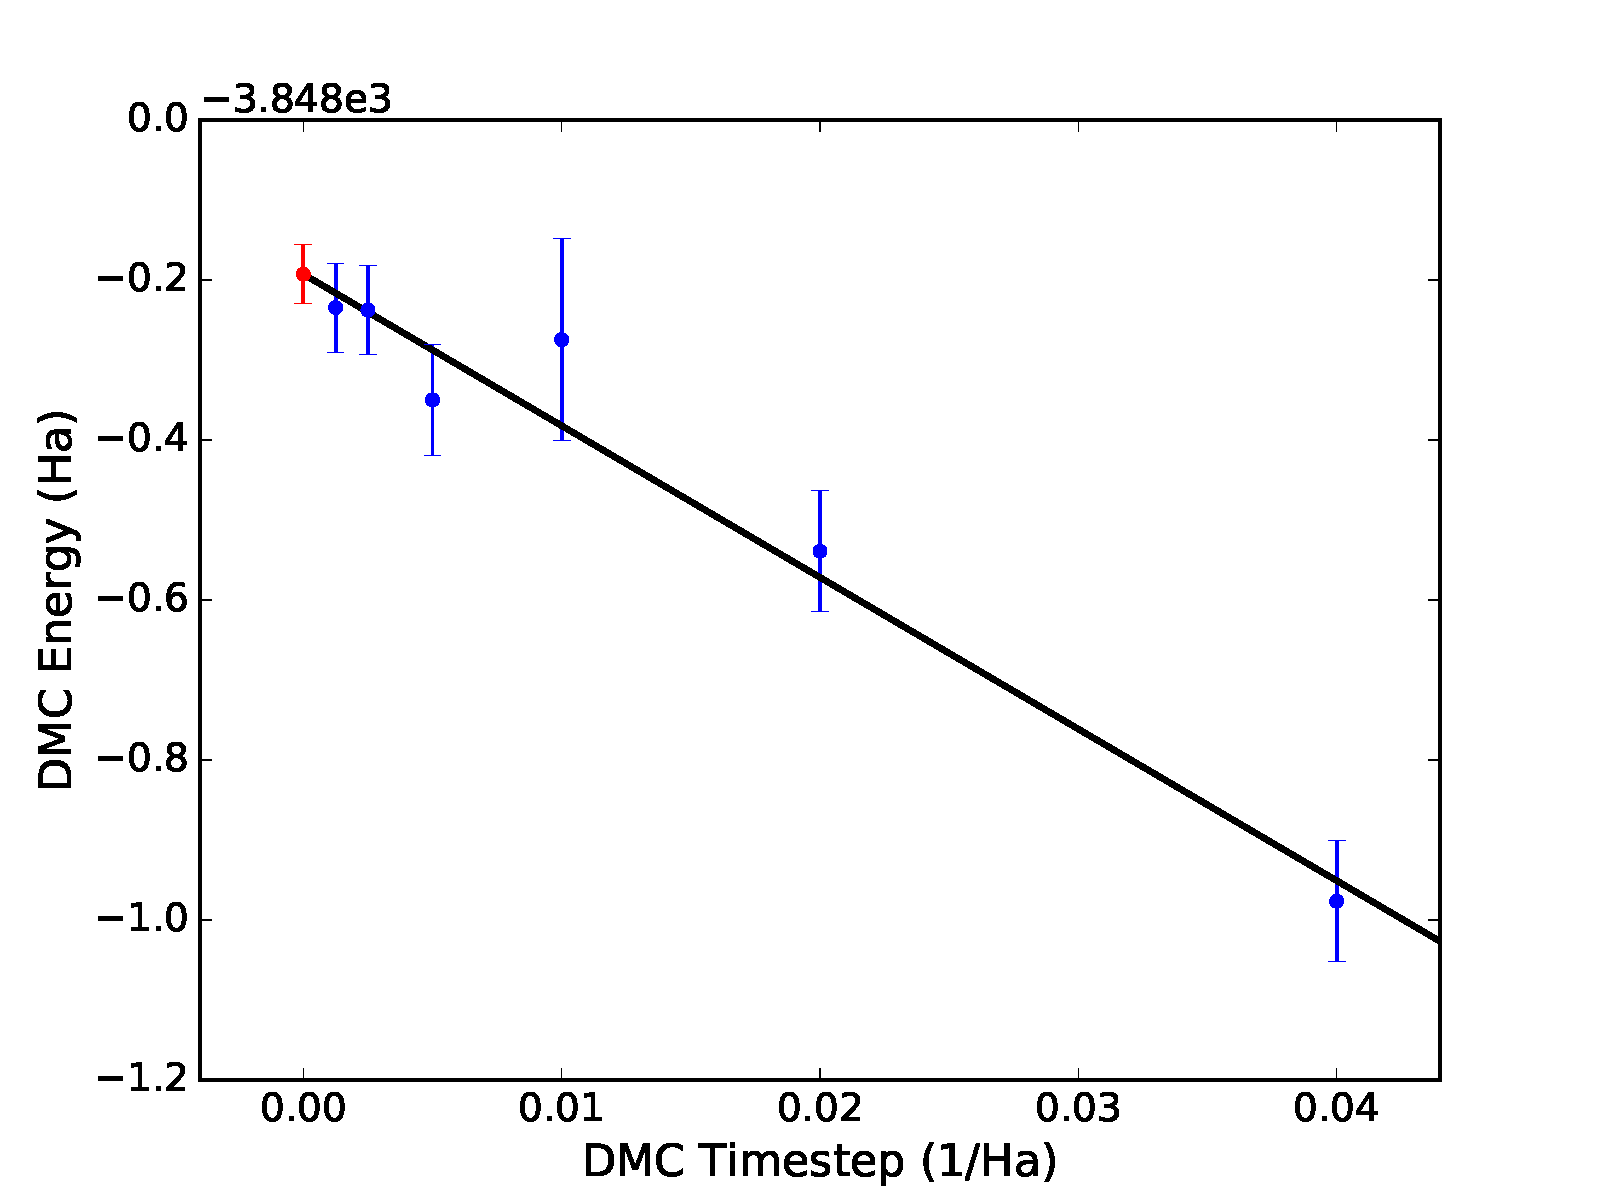
\includegraphics[trim=0mm 0mm 4mm 0mm,clip,width=512pt]{./figures/qmcfit_timestep_linear.dmn}&
    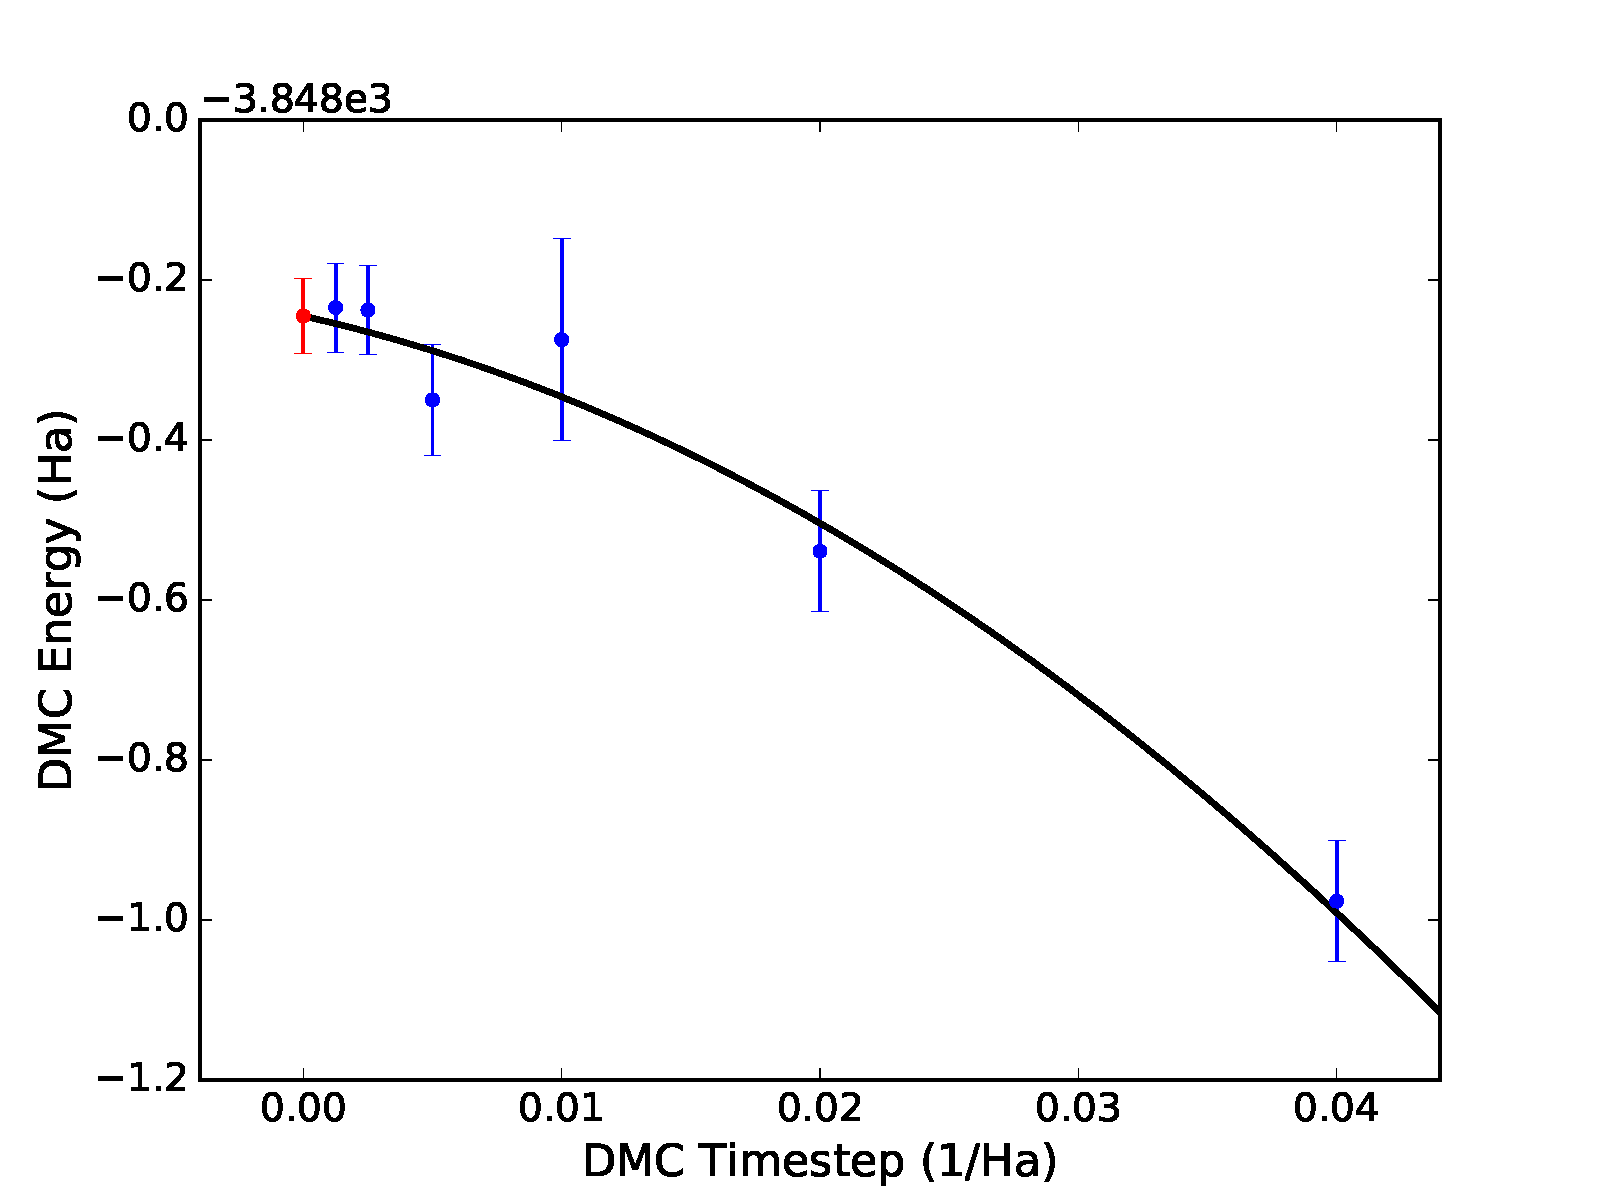
\includegraphics[trim=2mm 0mm 4mm 0mm,clip,width=512pt]{./figures/qmcfit_timestep_quadratic.dmn}\\
  \end{tabularx}
\else%
  \begin{tabularx}{\textwidth}{X X}
    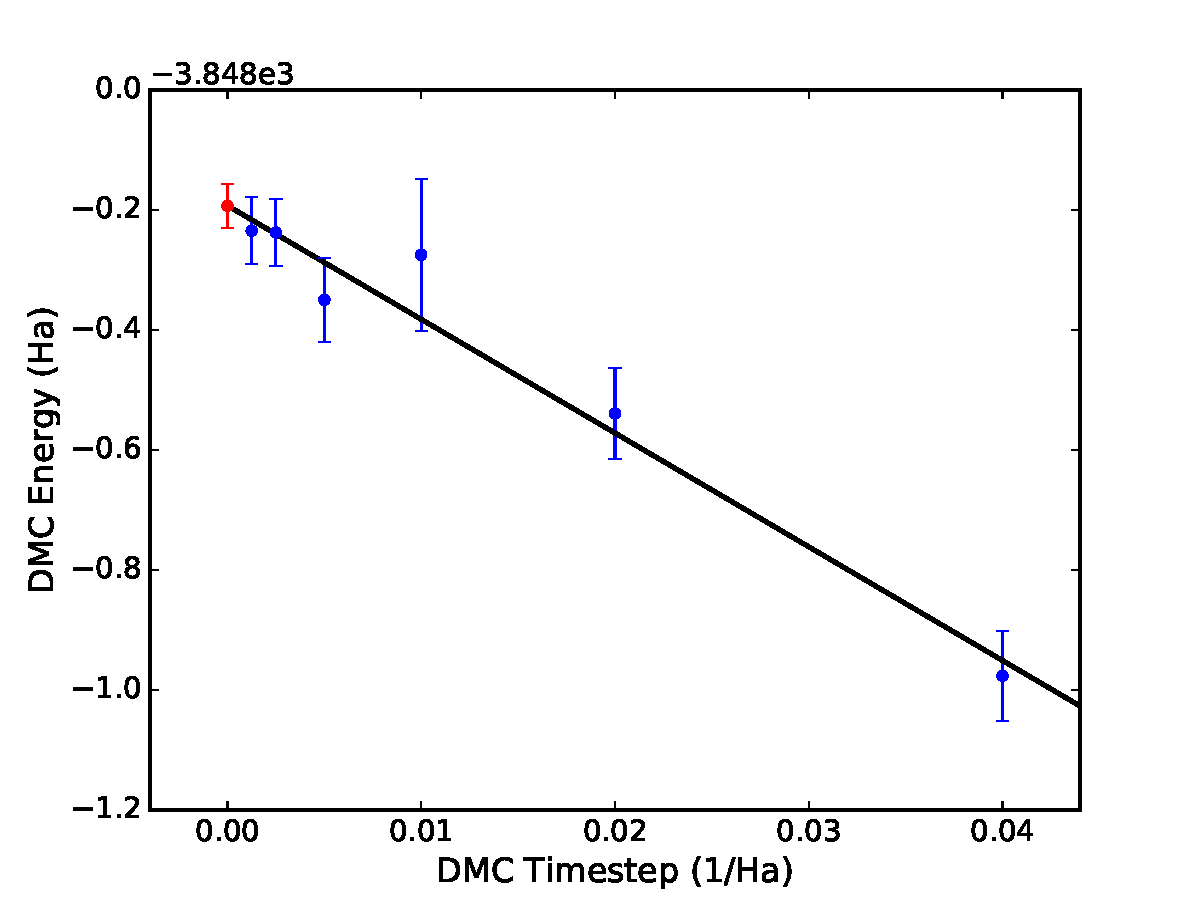
\includegraphics[trim=0mm 0mm 4mm 0mm,clip,width=0.47\textwidth]{./figures/qmcfit_timestep_linear.pdf}&
    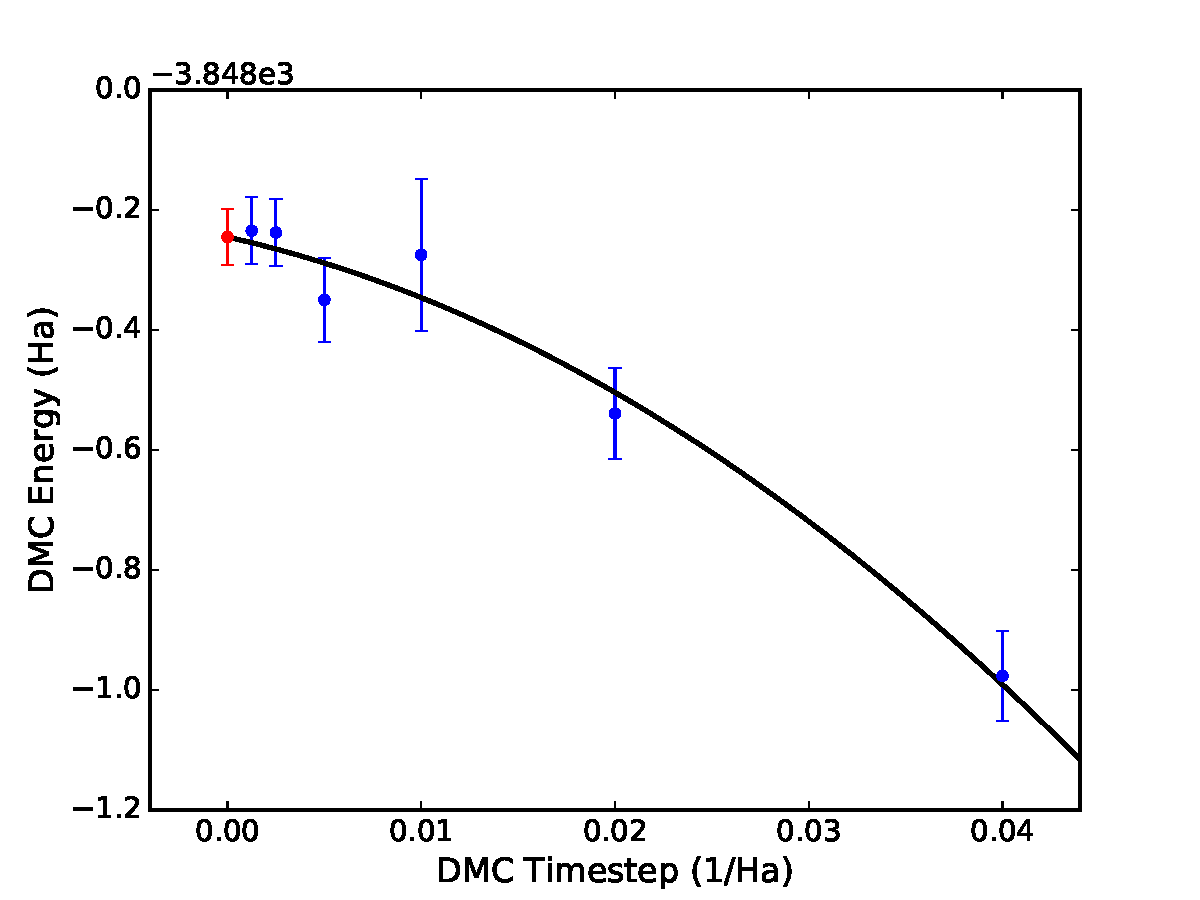
\includegraphics[trim=2mm 0mm 4mm 0mm,clip,width=0.47\textwidth]{./figures/qmcfit_timestep_quadratic.pdf}\\
    \end{tabularx}
\fi%
\caption{Linear (left) and quadratic (right) timestep fits to DMC data for a 32 atom supercell of MnO obtained with \texttt{qmc-fit}.  Zero timestep estimates are indicated by the red data point on the left side of either panel.}
  \label{fig:qmcfit_timestep}
\end{figure}

Different fitting functions are supported via the ``\texttt{-f}'' option.
Currently supported options include \texttt{linear} ($a+bt$),
\texttt{quadratic} ($a+bt+ct^2$), and \texttt{sqrt} ($a+b\sqrt{t}+ct$).
Results for a quadratic fit are shown below as well as in the right
panel of Fig.~\ref{fig:qmcfit_timestep}.
\begin{shade}
>qmc-fit ts -f quadratic -e30 -b4 -s2 -t '0.00125 0.0025 0.005 0.01 0.02 0.04' ./qmc*/*scalar*
fit function  : quadratic
fitted formula: (-3848.245 +/- 0.047) + (-7.25 +/- 8.33)*t + (-285.00 +/- 202.39)*t^2
intercept     : -3848.245 +/- 0.047  Ha
\end{shade}
In this case we find a zero timestep estimate of $-3848.25(5)$ Ha$^{-1}$.
A timestep of $0.04$ Ha$^{-1}$ might be on the large side to include in
timestep extrapolation and it is likely to have an outsize influence
in the case of linear extrapolation.  Upon excluding this point, linear
extrapolation yields a zero timestep value of $-3848.22(4)$ Ha$^{-1}$.
It should be noted that quadratic extrapolation can result in intrinsically
larger uncertainty in the extrapolated value.  For example, when the $0.04$
Ha$^{-1}$ point is excluded the uncertainty grows by 50\% and we obtain an
estimated value of $-3848.28(7)$ instead.



\section{Densities and spin-densities}
\label{sec:densities}
TBD.

%\section{Energy densities}
%\label{sec:energydensities}




